\documentclass{article}
\usepackage[english]{babel}

\usepackage[letterpaper,top=2cm,bottom=2cm,left=3cm,right=3cm,marginparwidth=1.75cm]{geometry}

\usepackage{amsmath, amsfonts, amsthm, amssymb, gensymb}
\usepackage{graphicx}

\PassOptionsToPackage{hyphens}{url}\usepackage[hidelinks]{hyperref}

% \usepackage{mathptmx}  % Times New Roman
% \usepackage{bookman}  % Bookman
% \usepackage{fourier}  % Fourier
\usepackage{tgpagella}  % TeX Gyre Pagella

\usepackage[usenames,dvipsnames, x11names,rgb]{xcolor}

\usepackage[skip=10pt plus1pt, indent=0pt]{parskip}

\usepackage[]{mdframed}  % For boxed text

\usepackage{easytable}

\usepackage{float}

\usepackage{tikz, pgfplots}
\pgfplotsset{compat=1.18}
\usepackage{tikz-3dplot}
\usetikzlibrary{calc}


\newcommand{\abs}[1]{|#1|}
\DeclareMathOperator{\kernel}{Ker}  % \ker exists but is lowercase
\DeclareMathOperator{\image}{Im}
\DeclareMathOperator{\Span}{Span}



\title{Introductory Mathematics for Computer Science (COMP0011)}
\author{Raphael Li}
\date{Year 1 Term 2, 2024--25}


\begin{document}
\maketitle

\vspace{1em}
\hrule
\vspace{1em}


\tableofcontents

\newpage
\section{Complex numbers}

The foundation of the \textit{complex numbers} is given by the imaginary unit \(i\), defined either as \(i = \sqrt{-1}\) or as \(i^2 = -1\).

A complex number \(z\) can be written as \(a + bi\), where \(a, b \in \mathbb{R}\). The real numbers \(a\) and \(b\) are known as the \textit{real part} and the \textit{complex part} of \(z\) respectively.

The set of all complex numbers is denoted as \(\mathbb{C}\). Note that the set of real numbers \(\mathbb{R}\) is a subset of \(\mathbb{C}\). See figure \ref{fig:Ch01-reals-in-complex}.


\begin{figure}[H]
    \centering
    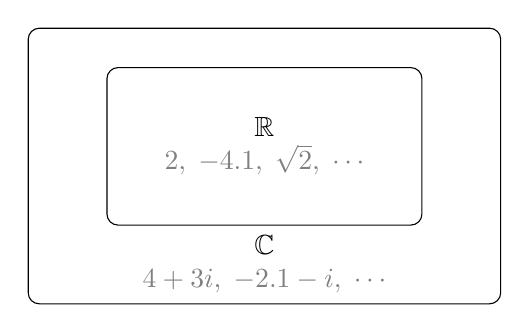
\begin{tikzpicture}
        \draw[rounded corners] (-2,0) rectangle (2,-2);

        \draw[rounded corners] (-3,0.5) rectangle (3,-3);

        \node[align=center] at (0,-1)  {\(\mathbb{R}\)\\ {\color{gray} \(2,\; -4.1,\; \sqrt{2},\; \cdots\)}};

        \node[align=center] at (0,-2.5)  {\(\mathbb{C}\)\\ {\color{gray} \(4+3i,\; -2.1-i,\; \cdots\)}};
    \end{tikzpicture}
    \caption{The set of real numbers \(\mathbb{R}\) is a subset of the set of complex numbers \(\mathbb{C}\). All real numbers are complex numbers.}
    \label{fig:Ch01-reals-in-complex}
\end{figure}





\subsection{Basic arithmetic with complex numbers, and complex conjugates}

To add or subtract two complex numbers, we deal with the real and imaginary parts separately.
%
\begin{align*}
    (2+3i) + (5-8i) &= (2+5) + (3 + (-8))i = 7 - 5i \tag{Addition}\\
    (2+3i) - (5-8i) &= (2-5) + (3 - (-8))i = -3 + 11i \tag{Subtraction}
\end{align*}

The multiplication of complex numbers is also straightforward as long as we bear in mind that \(i^2 = -1\).
%
\begin{align*}
    (3 + 4i)(-2 + 3i) &= -6 + 9i - 8i + 12i^2\\
    &= (-6-12) + (9-8)i\\
    &= -18 + i
\end{align*}

To divide a complex number by another, e.g.
%
\[\frac{a+bi}{c+di}\]
%
we multiply both the numerator and denominator by \(c - di\), which is obtained by flipping the sign of the imaginary part of the denominator. For example, if we want to compute
%
\[\frac{2+3i}{5-4i}\text{,}\]
%
we flip the sign of the imaginary part of \(5 - 4i\) to get \(5 + 4i\). We then multiply both the numerator and denominator of the fraction by this \(5 + 4i\) to get
%
\begin{align*}
    \frac{2+3i}{5-4i} &= \frac{(2+3i)(5 + 4i)}{(5-4i)(5 + 4i)}\\
    &= \frac{10 + 8i + 15i - 12}{25 + 20i - 20i + 16}\\
    &= \frac{-2 + 23i}{41}\\
    &= \frac{-2}{41} + \frac{23}{41}i \text{.}
\end{align*}

Notice how multiplying \(5 - 4i\) with \(5 + 4i\) produces the real number \(41\). By flipping the sign of the imaginary part of a complex number, we obtain what's called its \textit{complex conjugate}. The complex conjugate of \(z\) is denoted as \(\overline{z}\). By writing \(z\) as \(a + bi\), we can easily prove that the product of any complex number with its conjugate must equal a real number:
%
\[z \times \overline{z} = (a + bi)(a - bi) = a^2 + b^2 \in \mathbb{R}\text{.}\]





\subsection{Visualising complex numbers}

Given some complex number \(z = x + yi\), we can treat its real and imaginary parts as Cartesian coordinates, thus mapping it to a point on the 2D plane.

\begin{figure}[H]
    \centering

    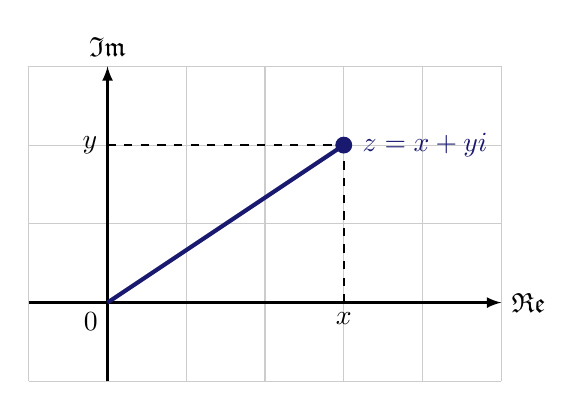
\begin{tikzpicture}
        \draw[thin,gray!40] (-1,-1) grid (5, 3);
        \draw[thick, ->, >=latex] (-1,0)--(5,0) node[right]{\(\mathfrak{Re}\)};
        \draw[thick, ->, >=latex] (0,-1)--(0,3) node[above]{\(\mathfrak{Im}\)};
        \draw (0, 0) node[below left] {\(0\)};
        
        \draw[dashed, thick] (3, 0) node[below]{\(x\)} --(3, 2);
        \draw[dashed, thick] (0, 2) node[left]{\(y\)} --(3, 2);

        \filldraw[radius=0.1, MidnightBlue] (3,2) circle;
        \draw[line width=1.5pt, MidnightBlue] (0,0)--(3,2) node[anchor=west]{\(\;z = x + yi\)};
    \end{tikzpicture}
    
    \caption{The complex number \(z = x + yi\) as a point on the 2D plane}
    \label{fig:02-ket-3-1}
\end{figure}



\subsection{Exponential form}

Recall that it is possible to express a point on a 2D plane using polar coordinates \((R, \theta)\) as well. Indeed, given any complex number \(z = x+yi\), we can find its corresponding pair of values \(R\) and \(\theta\).

\begin{figure}[H]
    \centering

    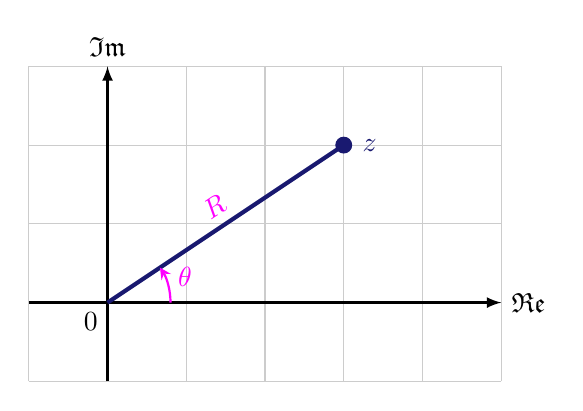
\begin{tikzpicture}
        \draw[thin,gray!40] (-1,-1) grid (5, 3);
        \draw[thick, ->, >=latex] (-1,0)--(5,0) node[right]{\(\mathfrak{Re}\)};
        \draw[thick, ->, >=latex] (0,-1)--(0,3) node[above]{\(\mathfrak{Im}\)};
        \draw (0, 0) node[below left] {\(0\)};

        \filldraw[radius=0.1, MidnightBlue] (3,2) circle;
        \draw[line width=1.5pt, MidnightBlue] (0,0)--(3,2) node[pos=0.5, sloped, anchor=south, Fuchsia]{\(R\)} node[anchor=west]{\(\;z\)};
        \draw[-stealth,Fuchsia, thick] (0.8, 0) arc (0:33.69:0.8) node[pos=0.5, anchor=west, shift={(0, 0.1)}]{\(\theta\)};
    \end{tikzpicture}
    
    \caption{The position of a complex number on the 2D plane can be represented using polar coordinates.}
    \label{fig:Ch01-complex-num-polar}
\end{figure}

Based on this idea, we introduce a new notation as follows.
%
\begin{quote}
    If the position of a complex number \(z\) on the 2D plane can be represented by the polar coordinates \((R, \theta)\), then we have
    %
    \[z = R \times e^{i\theta}\]
    %
    where \(R, \theta \in \mathbb{R}\) and \(R \geq 0\).

    \(R\) is called the \textit{absolute value} or \textit{modulus} of \(z\) and is denoted as \(\abs{z}\). This represents the point's position from the origin.

    \(\theta\) is called the \textit{argument} of \(z\) and is denoted as \(\arg(z)\). This represents the angle from horizontal.
\end{quote}
%
This way of representing complex numbers is known as the \textit{exponential form}. (This is a natural result of Euler's formula \(e^{i\theta} = \cos{\theta} + i\sin{\theta}\).)

Now consider two complex numbers expressed in exponential form.
%
\begin{align*}
    z_1 &= R_1 \times e^{i\theta_1}\\
    z_2 &= R_2 \times e^{i\theta_2}
\end{align*}
%
These two numbers are considered equal if both of the following conditions hold.
%
\begin{align*}
    R_1 &= R_2\\
    \theta_1 &= \theta_2 {\;\color{BrickRed} +2k\pi} \tag{for some \(k \in \mathbb{Z}\)}
\end{align*}
%
Note that the red part is necessary because a rotation of \(2\pi\) radians has no effect on a point's position.

The exponential form makes the multiplication and division of complex numbers a lot easier.

\begin{tabular}{c|c}
    \textbf{Multiplication} & \textbf{Division}\\
    \parbox{0.5\textwidth}{\centering
        \begin{align*}
            (1 \times e^{\frac{\pi}{6} i}) \times (2 \times e^{-\frac{\pi}{4} i}) &= 2 \times e^{\frac{\pi}{6} i -\frac{\pi}{4} i}\\
            &= 2 \times e^{-\frac{\pi}{12} i}
        \end{align*}
    }
    &
    \parbox{0.5\textwidth}{\centering
        \begin{align*}
            \frac{1 \times e^{\frac{\pi}{6} i}}{2 \times e^{-\frac{\pi}{4} i}} &= \frac{1}{2} \times \frac{e^{\frac{\pi}{6} i}}{e^{-\frac{\pi}{4} i}}\\
            &= 2 \times e^{\frac{5\pi}{12} i}
        \end{align*}
    }
\end{tabular}




\subsection{Converting between Cartesian and exponential forms}

The methods used to convert between the Cartesian form \(x + yi\) and the exponential form \(R \times e^{i\theta}\) are outlined below.
%
\begin{itemize}
    \item \textbf{Given the Cartesian form of a complex number, find its exponential form.}

    Given the Cartesian form \(z = x+yi\), we can find the modulus using Pythagoras' theorem.
    %
    \[\abs{z} = \sqrt{x^2 + y^2}\]
    %
    The argument can be found using the arctangent.
    %
    \[\arg(z) = \arctan\left(\frac{y}{x}\right)\]

    \item \textbf{Given the exponential form of a complex number, find its Cartesian form.}

    Given the exponential form \(z = R \times e^{i\theta}\), we can find the Cartesian coordinates using simple trigonometry.
    %
    \begin{align*}
        x &= R \cos{\theta}\\
        y &= R \sin{\theta}
    \end{align*}
\end{itemize}

To speed up conversion processes, it is often useful to memorize the Cartesian coordinates of some special points on the unit circle. See figure \ref{fig:Ch01-cartesian-coords-on-unit-circle} and table \ref{tab:Ch01-classic-angle-trig}.

\begin{figure}[H]
    \centering
    \includegraphics[width=0.6\linewidth]{Images/CartesianCoordsOnCircle.png}
    \caption{It is important to know the coordinates of points on the circle corresponding to classic angles.}
    \label{fig:Ch01-cartesian-coords-on-unit-circle}
\end{figure}

\begin{table}[H]
    \centering
    \begin{tabular}{|c||c|c|c|}
        \hline
        \(\theta\) (radians) & \(\pi/6\) & \(\pi/4\) & \(\pi/3\) \\
        \hline
        \(\theta\) (degrees) & \(30\degree\) & \(45\degree\) & \(60\degree\) \\
        \hline
        \(\sin{\theta}\) & \(\dfrac{1}{2}\) & \(\dfrac{\sqrt{2}}{2}\) & \(\dfrac{\sqrt{3}}{2}\)\\[1.5ex]
        \hline
        \(\cos{\theta}\) & \(\dfrac{\sqrt{3}}{2}\) & \(\dfrac{\sqrt{2}}{2}\) & \(\dfrac{1}{2}\)\\[1.5ex]
        \hline
    \end{tabular}
    \caption{The values of \(\sin{\theta}\) and \(\cos{\theta}\) for some classic angles \(\theta\).}
    \label{tab:Ch01-classic-angle-trig}
\end{table}




\subsection{Visualising arithmetic on complex numbers}

When visualised on the 2D plane, the addition of complex numbers is similar to that of vectors. We join the arrows in a tip-to-tail manner in order to determine the sum, as shown in figure \ref{fig:Ch01-adding-complex-numbers}.


\begin{figure}[H]
    \centering

    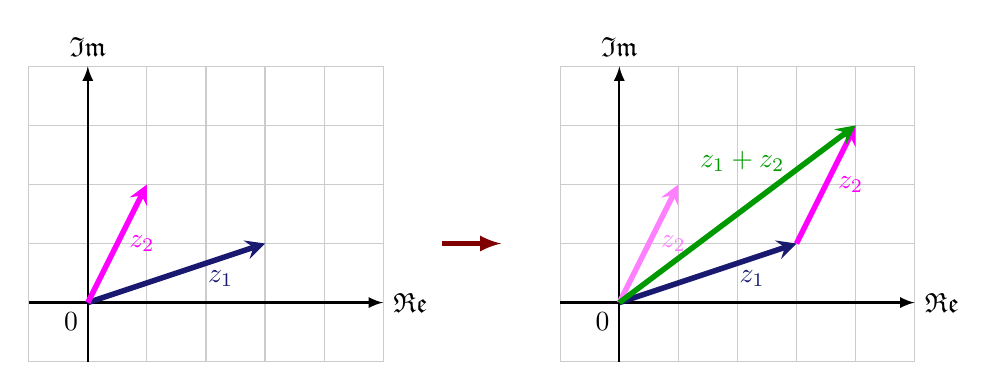
\begin{tikzpicture}[scale=0.75]
        \draw[thin,gray!40] (-1,-1) grid (5, 4);
        \draw[thick, ->, >=latex] (-1,0)--(5,0) node[right]{\(\mathfrak{Re}\)};
        \draw[thick, ->, >=latex] (0,-1)--(0,4) node[above]{\(\mathfrak{Im}\)};
        \draw (0, 0) node[below left] {0};
        
        \draw[line width=2pt, MidnightBlue, -stealth] (0,0)--(3,1) node[pos=3/4, below]{\(z_1\)};
        \draw[line width=2pt, Fuchsia, -stealth] (0,0)--(1,2) node[pos=1/2, anchor=west]{\(z_2\)};

        \draw[ultra thick, Maroon, ->, >=latex] (6, 1)--(7, 1);
        
        \begin{scope}[shift={(9, 0)}]
            \draw[thin,gray!40] (-1,-1) grid (5, 4);
            \draw[thick, ->, >=latex] (-1,0)--(5,0) node[right]{\(\mathfrak{Re}\)};
            \draw[thick, ->, >=latex] (0,-1)--(0,4) node[above]{\(\mathfrak{Im}\)};
            \draw (0, 0) node[below left] {0};
            
            \draw[line width=2pt, MidnightBlue, -stealth] (0,0)--(3,1) node[pos=3/4, below]{\(z_1\)};
            \draw[line width=2pt, Fuchsia!50, -stealth] (0,0)--(1,2) node[pos=1/2, anchor=west]{\(z_2\)};
            \draw[line width=2pt, Fuchsia, -stealth] (3,1)--(4,3) node[pos=1/2, anchor=west]{\(z_2\)};

            \draw[line width=2pt, OliveGreen, -stealth] (0,0)--(4,3) node[pos=3/4, anchor=east, shift={(0, 0.1)}]{\(z_1+z_2\)};
        \end{scope}
        
    \end{tikzpicture}
    
    \caption{Addition of complex numbers.}
    \label{fig:Ch01-adding-complex-numbers}
\end{figure}

The above figure also illustrates another key idea. Notice how in the figure on the right, the vectors of \(z_1\), \(z_2\) and \(z_1 + z_2\) form a triangle. This means their absolute values must fulfil the triangle inequality.
%
\[\abs{z_1} + \abs{z_2} \geq \abs{z_1+z_2}\]

To visualise multiplication we consider the exponential form. As shown in figure \ref{fig:Ch01-multiplying-complex-numbers}, when two complex numbers are multiplied, their arguments are added together to produce a rotation, while their moduli are multiplied.


\begin{figure}[H]
    \centering

    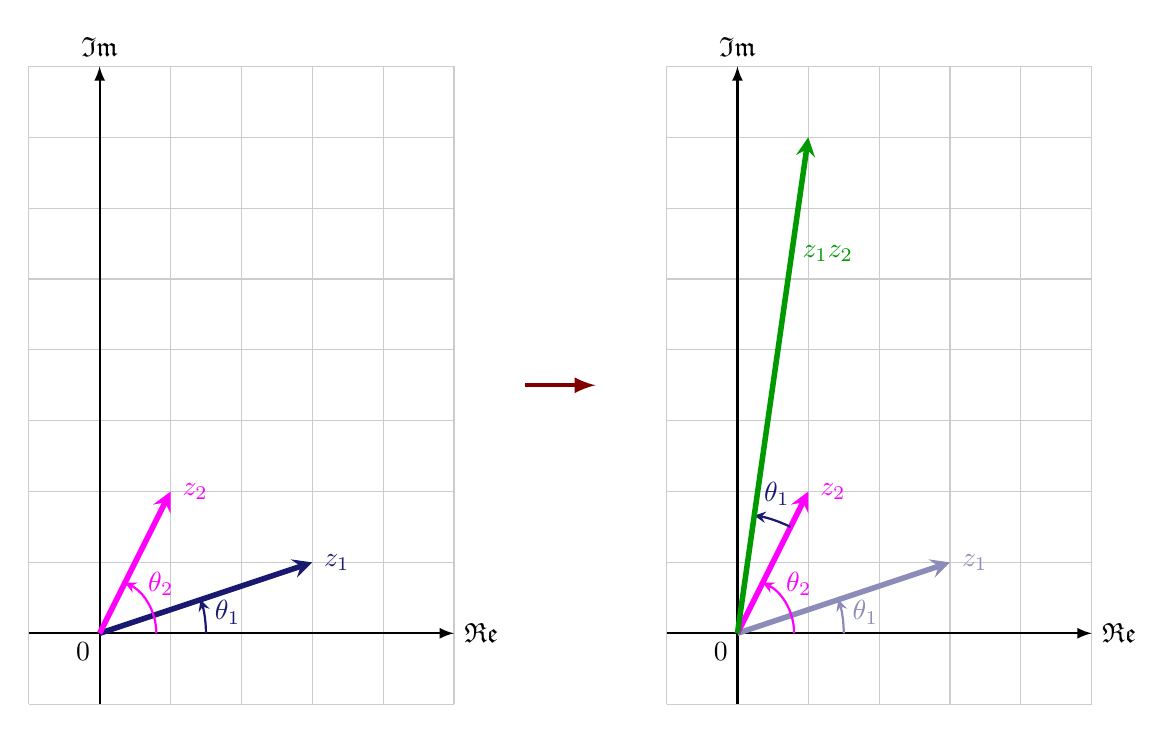
\begin{tikzpicture}[scale=0.9]
        \draw[thin,gray!40] (-1,-1) grid (5, 8);
        \draw[thick, ->, >=latex] (-1,0)--(5,0) node[right]{\(\mathfrak{Re}\)};
        \draw[thick, ->, >=latex] (0,-1)--(0,8) node[above]{\(\mathfrak{Im}\)};
        \draw (0, 0) node[below left] {0};
        
        \draw[line width=2pt, MidnightBlue, -stealth] (0,0)--(3,1) node[right]{\(z_1\)};
        \draw[-stealth, MidnightBlue, thick] (1.5, 0) arc (0:18.43:1.5) node[pos=0.5, anchor=west, shift={(0, 0.05)}]{\(\theta_1\)};
        
        \draw[line width=2pt, Fuchsia, -stealth] (0,0)--(1,2) node[right]{\(z_2\)};
        \draw[-stealth, Fuchsia, thick] (0.8, 0) arc (0:63.43:0.8) node[pos=0.75, anchor=west, shift={(0, 0.1)}]{\(\theta_2\)};

        \draw[ultra thick, Maroon, ->, >=latex] (6, 3.5)--(7, 3.5);
        
        \begin{scope}[shift={(9, 0)}]
            \draw[thin,gray!40] (-1,-1) grid (5, 8);
            \draw[thick, ->, >=latex] (-1,0)--(5,0) node[right]{\(\mathfrak{Re}\)};
            \draw[thick, ->, >=latex] (0,-1)--(0,8) node[above]{\(\mathfrak{Im}\)};
            \draw (0, 0) node[below left] {0};
            
            \draw[line width=2pt, MidnightBlue!50, -stealth] (0,0)--(3,1) node[right]{\(z_1\)};
            \draw[-stealth, MidnightBlue!50, thick] (1.5, 0) arc (0:18.43:1.5) node[pos=0.5, anchor=west, shift={(0, 0.05)}]{\(\theta_1\)};
            
            \draw[line width=2pt, Fuchsia, -stealth] (0,0)--(1,2) node[right]{\(z_2\)};
            \draw[-stealth, Fuchsia, thick] (0.8, 0) arc (0:63.43:0.8) node[pos=0.75, anchor=west, shift={(0, 0.1)}]{\(\theta_2\)};

            \draw[-stealth, MidnightBlue, thick] (0.75, 1.5) arc (63.43:63.43+18.43:1.677) node[pos=0.5, above, shift={(0.05, 0.05)}]{\(\theta_1\)};


            \draw[line width=2pt, OliveGreen, -stealth] (0,0)--(1,7) node[pos=3/4, anchor=west, shift={(0, 0.1)}]{\(z_1 z_2\)};
        \end{scope}
        
    \end{tikzpicture}
    
    \caption{Multiplication of complex numbers.}
    \label{fig:Ch01-multiplying-complex-numbers}
\end{figure}




\subsection{Roots of unity}

The \textit{roots of unity} are the solutions to the equation
%
\begin{equation}\label{eq:Ch01-roots-of-unity}
    z^n = 1\text{,}
\end{equation}
%
where \(n\) is a positive integer.

Solving this equation for values of \(n\) such as 2 and 4 is straightforward:
%
\begin{align*}
    n = 2 &\implies z^2 = 1 \implies z = 1 \text{ or } -1\\
    n = 4 &\implies z^4 = 1 \implies z = 1,\; i,\; -1 \text{ or } -i
\end{align*}
%
but solving it for other values of \(n\) requires us to express \(z\) in its exponential form, i.e.
%
\begin{equation}
    z = R \times e^{i\theta}\text{.} \tag{\(R, \theta \in \mathbb{R}\) and \(R\geq 0\)}
\end{equation}
%
This allows us to rewrite the equation as
%
\begin{align*}
    (R \times e^{i\theta})^n &= 1 \times e^{0i}\\
    R^n \times e^{in\theta} &= 1 \times e^{0i}
\end{align*}
%
which yields the following.
%
\[
\begin{cases}
    R^n = 1\\
    n\theta = 0 + 2k\pi = 2k\pi
\end{cases}
\tag{for some \(k \in \mathbb{Z}\)}
\]
%
Since \(R \geq 0\) and \(R \in \mathbb{R}\), we must have \(R = 1\). Furthermore, the second equation gives us
%
\[\theta = \frac{2k\pi}{n}\]
%
i.e.
%
\[\theta \in \left\{\cdots,\; -3\cdot\frac{2\pi}{n},\; -2\cdot\frac{2\pi}{n},\; -\frac{2\pi}{n},\; 0,\; \frac{2\pi}{n},\; 2\cdot \frac{2\pi}{n},\; 3\cdot\frac{2\pi}{n},\; \cdots\right\}\]
%
which seemingly means that there are infinitely many roots of unity. However, this is impossible because by the fundamental theorem of algebra, equation \eqref{eq:Ch01-roots-of-unity} (which is a polynomial equation of degree \(n\)) can only have \(n\) solutions.

To resolve this apparent paradox, let us visualise the problem on a 2D plane. For the sake of simplicity let us assume \(n = 3\). We know that all solutions to \eqref{eq:Ch01-roots-of-unity} must have a modulus of \(R = 1\), so they must lie on the unit circle.

\begin{figure}[H]
    \centering

    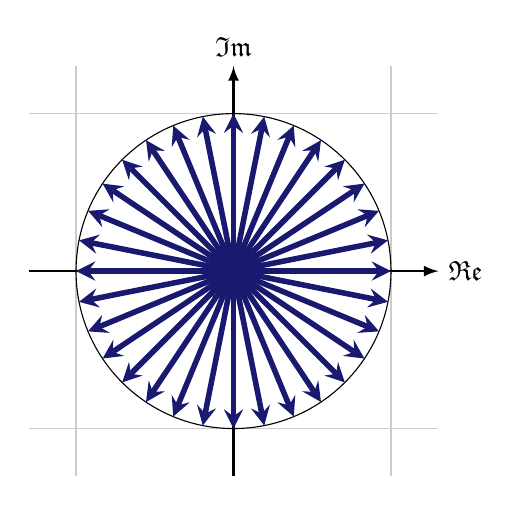
\begin{tikzpicture}[scale=2]
        \def\d{1.3}
        
        \draw[thin,gray!40] (-\d,-\d) grid (\d, \d);
        \draw[thick, ->, >=latex] (-\d,0)--(\d,0) node[right]{\(\mathfrak{Re}\)};
        \draw[thick, ->, >=latex] (0,-\d)--(0,\d) node[above]{\(\mathfrak{Im}\)};
        \draw (0, 0) node[below left] {0};

        \draw (0,0) circle [radius=1];
        
        \def\n{32}

        \foreach \i in {1,...,\n} {
            \draw[line width=2pt, MidnightBlue, -stealth] (0,0)--({cos(360/\n*\i)}, {sin(360/\n*\i)}) node {};
        }
    \end{tikzpicture}
    
    \caption{The roots of unity must lie somewhere on the unit circle.}
    \label{fig:Ch01-unit-circle}
\end{figure}

We want to find the angles \(\theta\) such that if we start at the point \(1\) and then rotate anticlockwise by \(\theta\) radians \(n = 3\) times, we end up back at \(1\).
%
\begin{itemize}
    \item Obviously we can have \(\theta = 0\).
    \item Another obvious solution is \(\theta = 2\pi/3\). If we rotate by this angle \(3\) times, we will have completed a full \(2\pi\) radians, bringing us back to the initial point.
    \item Moreover, we can also have \(\theta = 4\pi/3\). Rotating by this angle \(3\) times creates a total rotation of \(4\pi\) radians (i.e. 2 full cycles), bringing us once again back to the starting point.
    \item Continuing this pattern, it appears that \(\theta = 6\pi/3\) is also a solution. However, this is in fact the same as \(\theta = 0\), since angles differing by \(2\pi\) are considered equivalent. The same applies for \(\theta = 8\pi/3\) (equivalent to \(2\pi/3\)), \(\theta = 10\pi/3\) (equivalent to \(4\pi/3\)), and so on.
\end{itemize}

\begin{figure}[H]
    \centering

    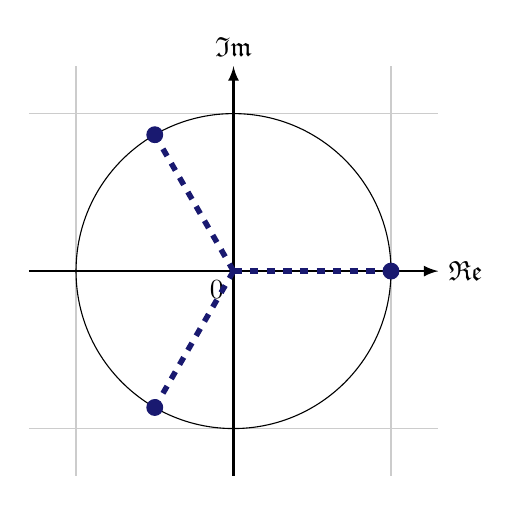
\begin{tikzpicture}[scale=2]
        \def\d{1.3}
        
        \draw[thin,gray!40] (-\d,-\d) grid (\d, \d);
        \draw[thick, ->, >=latex] (-\d,0)--(\d,0) node[right]{\(\mathfrak{Re}\)};
        \draw[thick, ->, >=latex] (0,-\d)--(0,\d) node[above]{\(\mathfrak{Im}\)};
        \draw (0, 0) node[below left] {0};

        \draw (0,0) circle [radius=1];
        
        \def\n{3}

        \foreach \i in {1,...,\n} {
            \filldraw[MidnightBlue] ({cos(360/\n*\i)}, {sin(360/\n*\i)}) circle [radius=0.05];

            \draw[line width=2pt, MidnightBlue, dashed] (0,0)--({cos(360/\n*\i)}, {sin(360/\n*\i)}) node {};
        }
    \end{tikzpicture}
    
    \caption{The third roots of unity.}
    \label{fig:Ch01-3rd-roots-of-unity}
\end{figure}

This resolves the above paradox --- we were right in thinking that the possible values of \(\theta\) are given by
%
\[\theta = \frac{2k\pi}{n}\]
%
or
%
\[\theta \in \left\{\cdots,\; -3\cdot\frac{2\pi}{n},\; -2\cdot\frac{2\pi}{n},\; -\frac{2\pi}{n},\; 0,\; \frac{2\pi}{n},\; 2\cdot \frac{2\pi}{n},\; 3\cdot\frac{2\pi}{n},\; \cdots\right\}\]
%
but these solutions are not all distinct. To make sure we only count distinct solutions, we impose the range \(0 \leq k < n\), giving us
%
\begin{equation}
    \theta = \frac{2k\pi}{n} \tag{\(k \in \mathbb{N}\) and \(k < n\)}
\end{equation}
%
or
%
\[\theta \in \left\{0,\; \frac{2\pi}{n},\; 2\cdot \frac{2\pi}{n},\; 3\cdot\frac{2\pi}{n},\; \cdots ,\; (n-1) \cdot\frac{2\pi}{n}\right\}\text{.}\]
%
This yields the solutions
%
\begin{equation}
    z = 1\times e^{\frac{2k\pi}{n}i} = e^{\frac{2k\pi}{n}i} \tag{\(k \in \mathbb{N}\) and \(k < n\)}
\end{equation}
or
%
\[z \in \left\{0,\; e^{\frac{2\pi}{n}i},\; e^{\frac{4\pi}{n}i},\; \cdots ,\; e^{\frac{2(n-1)\pi}{n}i}\right\}\text{.}\]







\newpage
\section{Continuous functions}

A function \(f\) maps elements of a set \(A\) to elements of another set \(B\). We denote this as \(f : A \rightarrow B\). In practice, most functions we consider will have type \(\mathbb{R} \rightarrow \mathbb{R}\).

If a function maps a number \(x\) to its square \(x^2\), we can denote this by \(x \mapsto x^2\). (Note the difference in the arrow symbol used --- the symbol \(\mapsto\) is read as ``maps to''.)

A function \(y = f(x)\) can be represented graphically as the set of points \((x, y)\). See figure \ref{fig:Ch02-quadratic-graph}.

\begin{figure}[H]
    \centering

    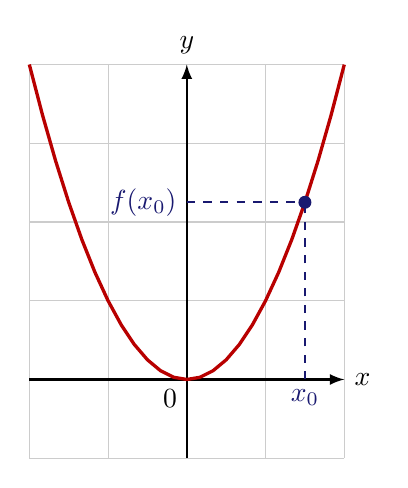
\begin{tikzpicture}
        \draw[thin,gray!40] (-2,-1) grid (2, 4);
        \draw[thick, ->, >=latex] (-2,0)--(2,0) node[right]{\(x\)};
        \draw[thick, ->, >=latex] (0,-1)--(0,4) node[above]{\(y\)};
        \draw (0, 0) node[below left] {0};

        \draw [BrickRed, very thick, domain=-2:2] plot (\x, {\x*\x}); 

        \draw[MidnightBlue, dashed, thick] (1.5, 0) node[below]{\(x_0\)} --(1.5, 2.25);
        \draw[MidnightBlue, dashed, thick] (0, 2.25) node[left]{\(f(x_0)\)} --(1.5, 2.25);

        \filldraw[radius=0.075, MidnightBlue] (1.5,2.25) circle;
    \end{tikzpicture}
    
    \caption{The graph of the function \(y = x^2\).}
    \label{fig:Ch02-quadratic-graph}
\end{figure}

In the next few subsections, we will be looking at some classic mathematical functions.


\subsection{Trigonometric functions}

Consider a point \(P\) on the unit circle. If we let \(\theta\) be the angle between \(OP\) and the horizontal axis, then the coordinates of \(P\) can be expressed as \((\cos{\theta},\; \sin{\theta})\). This is illustrated in figure \ref{fig:Ch02-trig-funcs-on-unit-circle}.

\begin{figure}[H]
    \centering

    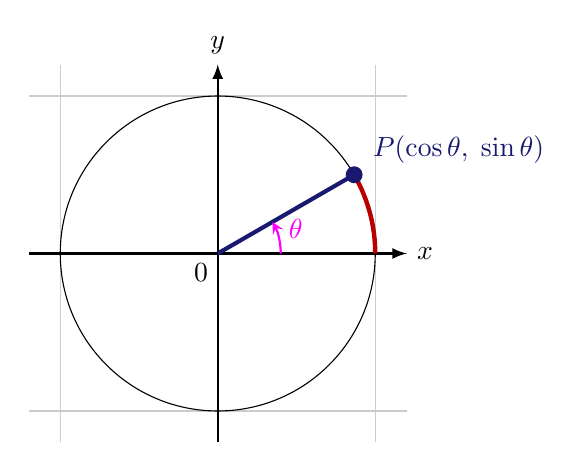
\begin{tikzpicture}[scale=2]
        \draw[thin,gray!40] (-1.2,-1.2) grid (1.2, 1.2);

        \draw[radius=1] (0, 0) circle;

        \draw[thick, ->, >=latex] (-1.2,0)--(1.2,0) node[right]{\(x\)};
        \draw[thick, ->, >=latex] (0,-1.2)--(0,1.2) node[above]{\(y\)};
        \draw (0, 0) node[below left] {\(0\)};

        \draw[BrickRed, ultra thick] (1, 0) arc (0:30:1);

        \filldraw[radius=0.05, MidnightBlue] ({sqrt(3)/2}, 0.5) circle;
        \draw[line width=1.5pt, MidnightBlue] (0,0)--({sqrt(3)/2}, 0.5) node[anchor=south west]{\(\;P(\cos{\theta},\; \sin{\theta})\)};
        \draw[-stealth,Fuchsia, thick] (0.4, 0) arc (0:30:0.4) node[pos=0.5, anchor=west, shift={(0, 0.1)}]{\(\theta\)};

        
    \end{tikzpicture}
    
    \caption{The trigonometric functions \(\cos{\theta}\) and \(\sin{\theta}\) can be defined using the unit circle. Note that if we are measuring \(\theta\) in radians, then the length of the arc highlighted in red must be equal to \(\theta\).}
    \label{fig:Ch02-trig-funcs-on-unit-circle}
\end{figure}

We've previously seen the values of \(\sin{\theta}\) and \(\cos{\theta}\) for some classic angles \(\theta\) in table \ref{tab:Ch01-classic-angle-trig}. Plotting these functions on a graph results in figure \ref{fig:Ch02-trig-funcs-graph}.

\begin{figure}[H]
    \centering

    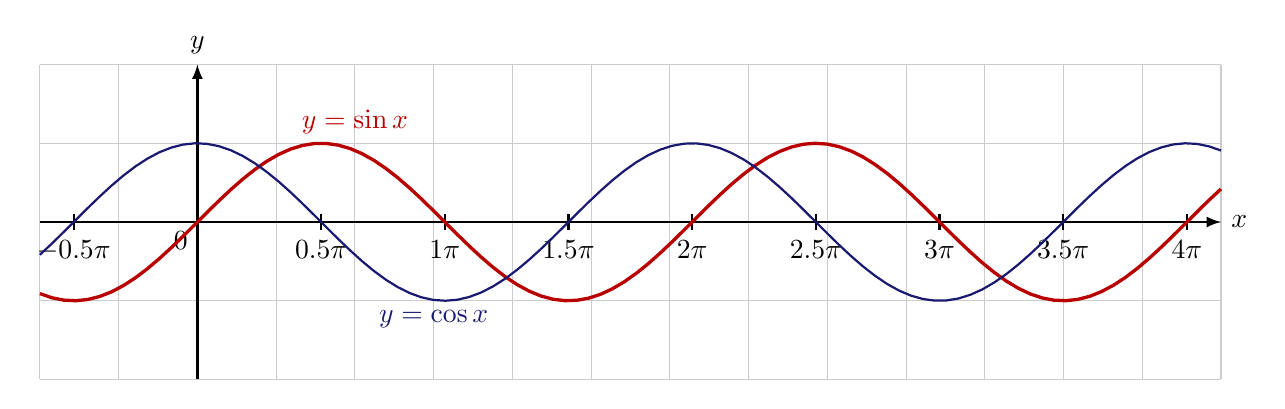
\begin{tikzpicture}
        \draw[thin,gray!40] (-2,-2) grid (13, 2);
        \draw[thick, ->, >=latex] (-2,0)--(13,0) node[right]{\(x\)};
        \draw[thick, ->, >=latex] (0,-2)--(0,2) node[above]{\(y\)};
        \draw (0, 0) node[below left] {0};

        \foreach \x in {-0.5, 0.5, 1, ..., 4} {
            \draw[thick] (\x*3.14159, 0.1) -- (\x*3.14159, -0.1) node[below] {\(\x\pi\)};
        }

        % \x r means to convert '\x' from degrees to radians:
        \draw [BrickRed, very thick, domain=-2:13, samples=100] plot (\x,{sin(\x r)});

        \draw [MidnightBlue, thick, domain=-2:13, samples=100] plot (\x,{cos(\x r)});

        \draw node[BrickRed, above] at (2, 1) {\(y = \sin{x}\)};
        \draw node[MidnightBlue, below] at (3, -1) {\(y = \cos{x}\)};
    \end{tikzpicture}
    
    \caption{The graph of the functions \(\sin{x}\) and \(\cos{x}\).}
    \label{fig:Ch02-trig-funcs-graph}
\end{figure}





\subsection{Exponential and logarithm}

One way to define the exponential function \(\exp\) is as follows.
%
\begin{align*}
    \exp(x + y) &= \exp(x) \cdot \exp(y)\\
    \exp(0) &= 1\\
    \frac{d}{dx} \exp(x) &= \exp(x) 
\end{align*}
%
Note that the first two relationships can be satisfied by any function of the form \(f(x) = a^x\) where \(a \in \mathbb{R}\). However, if we take all three conditions into account, the only function satisfying them is \(\exp(x) = e^x\), where \(e = 2.71828\cdots\) is Euler's number.

The exponential function \(\exp(x) = e^x\) is plotted in figure \ref{fig:Ch02-exp-graph}. Note that:
%
\begin{itemize}
    \item For all values of \(x\), we have \(\exp(x) > 0\).
    \item When \(x\) is negative, \(\exp(x)\) is very small.
    \item The value of \(\exp(x)\) grows very fast as \(x\) increases.
\end{itemize}

\begin{figure}[H]
    \centering

    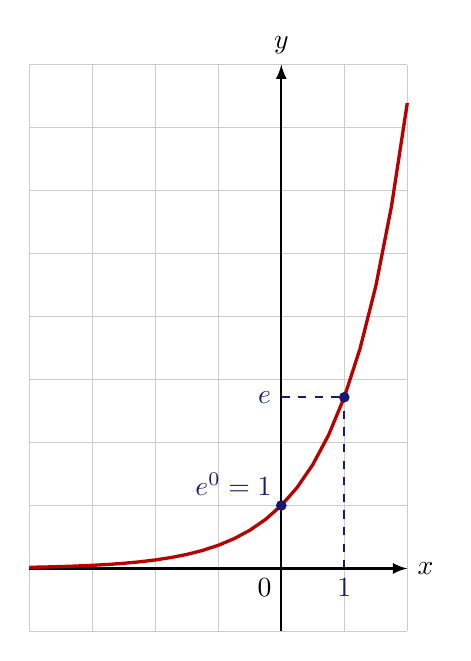
\begin{tikzpicture}[scale=0.8]
        \draw[thin,gray!40] (-4,-1) grid (2, 8);
        \draw[thick, ->, >=latex] (-4,0)--(2,0) node[right]{\(x\)};
        \draw[thick, ->, >=latex] (0,-1)--(0,8) node[above]{\(y\)};
        \draw (0, 0) node[below left] {0};

        \draw [BrickRed, very thick, domain=-4:2] plot (\x, {2.71828^\x}); 
        \filldraw[radius=0.075, MidnightBlue] (0,1) circle node[above left] {\(e^0 = 1\)};

        \draw[MidnightBlue, dashed, thick] (1, 0) node[below]{\(1\)} --(1, 2.71828);
        \draw[MidnightBlue, dashed, thick] (0, 2.71828) node[left]{\(e\)} --(1, 2.71828);

        \filldraw[radius=0.075, MidnightBlue] (1, 2.71828) circle;
    \end{tikzpicture}
    
    \caption{The graph of the function \(y = \exp(x) = e^x\).}
    \label{fig:Ch02-exp-graph}
\end{figure}

The natural logarithm \(\ln{x}\) is the inverse of the exponential, meaning that \(\ln(e^x) = x\). This results in the following properties.
%
\begin{align*}
    \ln(ab) &= \ln{a} + \ln{b}\\
    \ln\left(\frac{a}{b}\right) &= \ln{a} - \ln{b}\\
    \ln{1} &= 0\\
    \ln{e} &= 1\\
    a^x &= e^{x\ln{a}}\\
    \ln(a^x) &= x\ln{a}
\end{align*}
%
Since \(e^x > 0\) for all \(x\), the natural logarithm \(\ln{x}\) is only defined for positive values of \(x\).

The plot of \(y = \ln{x}\) is given in figure \ref{fig:Ch02-ln-graph}. Note that:
%
\begin{itemize}
    \item For \(x < 1\), we have \(\ln{x} < 0\).
    \item The curve intersects the \(x\)-axis at \((1, 0)\).
    \item For \(x > 1\), the value of \(\ln{x}\) grows very slowly as \(x\) increases.
\end{itemize}

\begin{figure}[H]
    \centering

    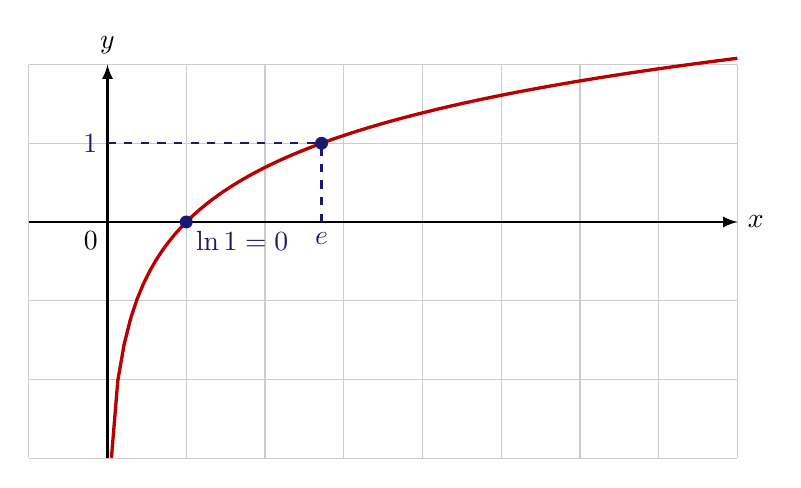
\begin{tikzpicture}
        \draw[thin,gray!40] (-1,-3) grid (8, 2);
        \draw[thick, ->, >=latex] (-1,0)--(8,0) node[right]{\(x\)};
        \draw[thick, ->, >=latex] (0,-3)--(0,2) node[above]{\(y\)};
        \draw (0, 0) node[below left] {0};

        \draw [BrickRed, very thick, domain=0.05:8, samples=100] plot (\x, {ln(\x)}); 
        \filldraw[radius=0.075, MidnightBlue] (1, 0) circle node[below right] {\(\ln{1} = 0\)};

        \draw[MidnightBlue, dashed, thick] (0, 1) node[left]{\(1\)} --(2.71828, 1);
        \draw[MidnightBlue, dashed, thick] (2.71828, 0) node[below]{\(e\)} --(2.71828, 1);

        \filldraw[radius=0.075, MidnightBlue] (2.71828, 1) circle;
    \end{tikzpicture}
    
    \caption{The graph of the function \(y = \exp(x) = e^x\).}
    \label{fig:Ch02-ln-graph}
\end{figure}




\subsection{Introduction to limits}

The idea of limits is simple.
%
\begin{quote}
    As the input \(x\) approaches a value \(p\), the output \(f(x)\) also approaches a value \(L\). (Both \(p\) and \(L\) possibly infinite.) To denote this we write \(f(x) \rightarrow L\) as \(x \rightarrow p\), or \(\lim_{x \rightarrow p} f(x) = L\).
\end{quote}

How do you formally define something like that?

Let us consider the simplest case, where both \(p\) and \(L\) are finite. We give the following definition.
%
\begin{quote}
    \textbf{Definition of a limit, with both \(p\) and \(L\) finite.}

    The main idea is that \(f(x)\) can get \textit{arbitrarily close} to \(L\) as long as \(x\) is close enough to \(p\).

    In other words, {\color{BrickRed} no matter how close we want our output to be to \(L\)}, {\color{Fuchsia} we can always find a range of inputs around \(p\)} such that {\color{MidnightBlue} the output is within that range}. This is written as
    %
    \[
    {\color{BrickRed} \forall \epsilon > 0},\;
    {\color{Fuchsia} \exists \delta > 0},\;
    {\color{Fuchsia} \forall x \in \mathbb{R}},\;
    {\color{Fuchsia} 0 < \abs{x - p} < \delta}
    \Rightarrow
    {\color{MidnightBlue} \abs{f(x) - L} < \epsilon}
    \text{.}
    \]
\end{quote}
%
This is called the epsilon-delta or \((\epsilon, \delta)\) definition of a limit. See figure \ref{fig:Ch02-lim-val-val} for an illustration of this.

\begin{figure}[H]
    \centering

    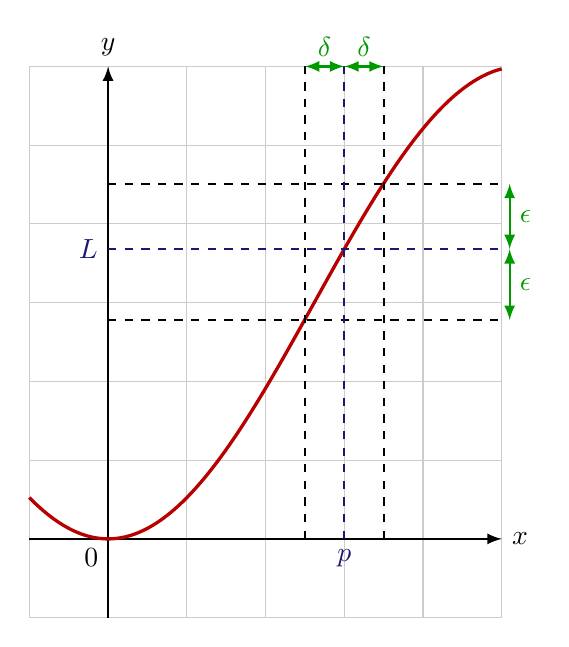
\begin{tikzpicture}
        \draw[thin,gray!40] (-1,-1) grid (5, 6);
        \draw[thick, ->, >=latex] (-1,0)--(5,0) node[right]{\(x\)};
        \draw[thick, ->, >=latex] (0,-1)--(0,6) node[above]{\(y\)};
        \draw (0, 0) node[below left] {0};

        \draw [BrickRed, very thick, domain=-1:5, samples=100] plot (\x, {6*(sin((0.3*\x) r))^2}); 

        \draw[dashed, thick] (0, 2.78) -- (5, 2.78);
        \draw[dashed, thick] (0, 4.51) -- (5, 4.51);

        \draw[dashed, thick] (2.5, 0) -- (2.5, 6);
        \draw[dashed, thick] (3.5, 0) -- (3.5, 6);

        \draw[MidnightBlue, dashed, thick] (3, 0) node[below]{\(p\)} -- (3, 6);
        \draw[MidnightBlue, dashed, thick] (0, 3.68) node[left]{\(L\)} -- (5, 3.68);

        \draw[OliveGreen, thick, latex-latex] (2.5, 6) -- (3, 6) node[pos=0.5, above] {\(\delta\)};

        \draw[OliveGreen, thick, latex-latex] (3, 6) -- (3.5, 6) node[pos=0.5, above] {\(\delta\)};

        \draw[OliveGreen, thick, latex-latex, shift={(0.1, 0)}] (5, 2.78) -- (5, 3.68) node[pos=0.5, right] {\(\epsilon\)};

        \draw[OliveGreen, thick, latex-latex, shift={(0.1, 0)}] (5, 3.68) -- (5, 4.51) node[pos=0.5, right] {\(\epsilon\)};
    \end{tikzpicture}
    
    \caption{As \(x\) approaches \(p\), \(f(x)\) approaches \(L\).}
    \label{fig:Ch02-lim-val-val}
\end{figure}


An example problem utilising the definition is shown below.

\vspace{15pt}
\begin{mdframed}[linewidth=1pt]
\noindent \textbf{Problem.} Using the epsilon-delta definition of a limit, show that \(\lim_{x \rightarrow 2} 2x + 3 = 7\).

\vspace{10pt}

\textbf{Intuition.} We want to show that
%
\[\forall \epsilon > 0,\; \exists \delta > 0,\; \forall x \in \mathbb{R},\; 0 < \abs{x - 2} < \delta \Rightarrow \abs{2x + 3 - 7} < \epsilon\]
%
i.e.
%
\[\forall \epsilon > 0,\; \exists \delta > 0,\; \forall x \in \mathbb{R},\; 0 < \abs{x - 2} < \delta \Rightarrow \abs{2x - 4} < \epsilon\]

Given some \(\epsilon > 0\), we need to work out how to choose a \(\delta\) value such that \(0 < \abs{x - 2} < \delta\) implies \(\abs{2x - 4} < \epsilon\). Simple observation shows that we can choose \(\delta = \epsilon/2\), which allows us to construct the proof below.

\vspace{10pt}

\textbf{Proof.} We want to show that
%
\[\forall \epsilon > 0,\; \exists \delta > 0,\; \forall x \in \mathbb{R},\; 0 < \abs{x - 2} < \delta \Rightarrow \abs{2x - 4} < \epsilon\text{.}\]
%
For any \(\epsilon > 0\), let \(\delta = \epsilon/2 > 0\). Then if \(0 < \abs{x - 2} < \delta\) for some real \(x\), we have
%
\begin{align*}
    \abs{x - 2} &< \delta\\
    \abs{x - 2} &< \frac{\epsilon}{2}\\
    2\abs{x - 2} &< \epsilon\\
    \abs{2x - 4} &< \epsilon
\end{align*}
%
which concludes the proof.
\end{mdframed}
\vspace{15pt}


Now, what happens if \(L\) is infinite? We can define this as follows.
%
\begin{quote}
    \textbf{Definition of a limit, with \(p\) finite and \(L\) infinite.}

    The main idea is that \(f(x)\) can become arbitrarily large as \(x\) gets close enough to \(p\).

    In other words, {\color{BrickRed} for any value \(d\)}, {\color{Fuchsia} we can always find a range of inputs around \(p\)} such that {\color{MidnightBlue} the output is greater than \(d\)}. This is written as
    %
    \[
    {\color{BrickRed} \forall d > 0},\;
    {\color{Fuchsia} \exists \delta > 0},\;
    {\color{Fuchsia} \forall x \in \mathbb{R}},\;
    {\color{Fuchsia} 0 < \abs{x - p} < \delta}
    \Rightarrow
    {\color{MidnightBlue} f(x) > d}
    \text{.}
    \]
\end{quote}
%
See figure \ref{fig:Ch02-lim-val-inf}.


\begin{figure}[H]
    \centering

    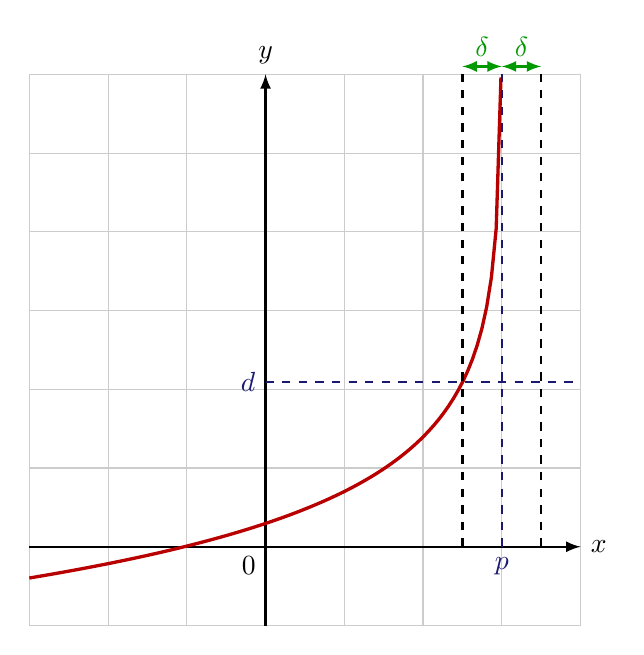
\begin{tikzpicture}
        \draw[thin,gray!40] (-3,-1) grid (4, 6);
        \draw[thick, ->, >=latex] (-3,0)--(4,0) node[right]{\(x\)};
        \draw[thick, ->, >=latex] (0,-1)--(0,6) node[above]{\(y\)};
        \draw (0, 0) node[below left] {0};

        \draw [BrickRed, very thick, domain=-3:2.99, samples=100] plot (\x, {6-ln(300-100*\x)}); 

        \draw[dashed, thick] (2.5, 0) -- (2.5, 6);
        \draw[dashed, thick] (3.5, 0) -- (3.5, 6);
        \draw[MidnightBlue, dashed, thick] (0, 2.09) node[left]{\(d\)} -- (4, 2.09);

        \draw[MidnightBlue, thick, dashed] (3, 0) node[below]{\(p\)} -- (3, 6);

        \draw[OliveGreen, thick, latex-latex, shift={(0, 0.1)}] (2.5, 6) -- (3, 6) node[pos=0.5, above] {\(\delta\)};

        \draw[OliveGreen, thick, latex-latex, shift={(0, 0.1)}] (3, 6) -- (3.5, 6) node[pos=0.5, above] {\(\delta\)};
    \end{tikzpicture}
    
    \caption{As \(x\) approaches \(p\), \(f(x)\) approaches infinity.}
    \label{fig:Ch02-lim-val-inf}
\end{figure}


Now let us consider the opposite scenario where \(L\) is finite but \(p\) is infinite. We modify our definition like so.
%
\begin{quote}
    \textbf{Definition of a limit, with \(p\) infinite and \(L\) finite.}

    The main idea is that \(f(x)\) can become arbitrarily close to \(L\) as long as \(x\) is large enough.

    In other words, {\color{BrickRed} no matter how close we want our output to be to \(L\)}, {\color{Fuchsia} we can always find a value \(c\)} such that {\color{Fuchsia} as long as \(x\) is greater than \(c\)}, {\color{MidnightBlue} the output is within that range}. This is written as
    %
    \[
    {\color{BrickRed}\forall \epsilon > 0},\;
    {\color{Fuchsia} \exists c > 0},\;
    {\color{Fuchsia} \forall x \in \mathbb{R}},\;
    {\color{Fuchsia} x > c}
    \Rightarrow
    {\color{MidnightBlue} \abs{f(x) - L} < \epsilon}
    \text{.}
    \]
\end{quote}
%
See figure \ref{fig:Ch02-lim-inf-val}.


\begin{figure}[H]
    \centering

    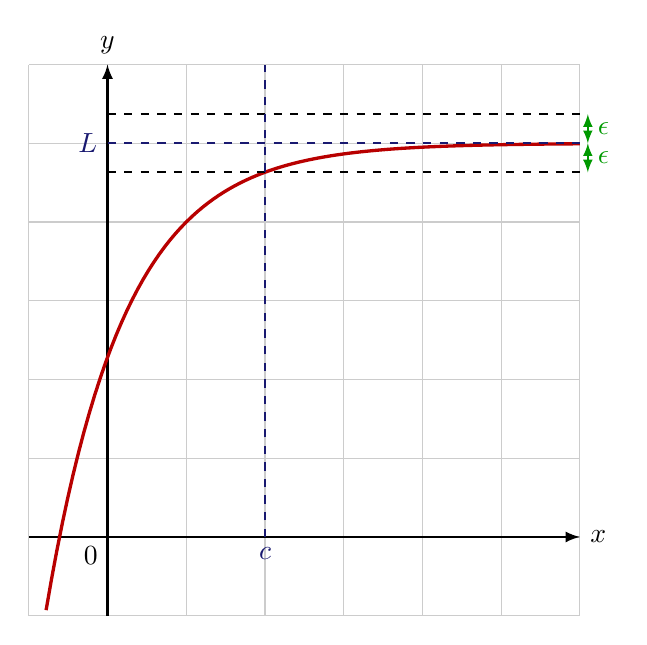
\begin{tikzpicture}
        \draw[thin,gray!40] (-1,-1) grid (6, 6);
        \draw[thick, ->, >=latex] (-1,0)--(6,0) node[right]{\(x\)};
        \draw[thick, ->, >=latex] (0,-1)--(0,6) node[above]{\(y\)};
        \draw (0, 0) node[below left] {0};

        \draw [BrickRed, very thick, domain=-0.78:6, samples=100] plot (\x, {5-2.71828^(1-\x)}); 

        \draw[dashed, thick] (0, 4.63) -- (6, 4.63);
        \draw[dashed, thick] (0, 5.37) -- (6, 5.37);
        \draw[MidnightBlue, dashed, thick] (2, 0) node[below]{\(c\)} -- (2, 6);

        \draw[MidnightBlue, thick, dashed] (0, 5) node[left]{\(L\)}-- (6, 5);

        \draw[OliveGreen, semithick, latex-latex, shift={(0.1, 0)}] (6, 5.37) -- (6, 5) node[pos=0.5, right] {\(\epsilon\)};

        \draw[OliveGreen, semithick, latex-latex, shift={(0.1, 0)}] (6, 5) -- (6, 4.63) node[pos=0.5, right] {\(\epsilon\)};
    \end{tikzpicture}
    
    \caption{As \(x\) approaches infinity, \(f(x)\) approaches \(L\).}
    \label{fig:Ch02-lim-inf-val}
\end{figure}



The final case is where both \(p\) and \(L\) are infinite. The definition for this is as follows.
%
\begin{quote}
    \textbf{Definition of a limit, with both \(p\) and \(L\) infinite.}

    The main idea is that \(f(x)\) can become arbitrarily large as \(x\) gets large enough.

    In other words, {\color{BrickRed} for any value \(d\)}, {\color{Fuchsia} we can always find a value \(c\)} such that {\color{Fuchsia} as long as \(x\) is greater than \(c\)}, {\color{MidnightBlue} the output is greater than \(d\)}. This is written as
    %
    \[
    {\color{BrickRed} \forall d > 0},\;
    {\color{Fuchsia} \exists c > 0},\;
    {\color{Fuchsia} \forall x \in \mathbb{R}},\;
    {\color{Fuchsia} x > c}
    \Rightarrow
    {\color{MidnightBlue} f(x) > d}
    \text{.}
    \]
\end{quote}

See figure \ref{fig:Ch02-lim-inf-inf}.


\begin{figure}[H]
    \centering

    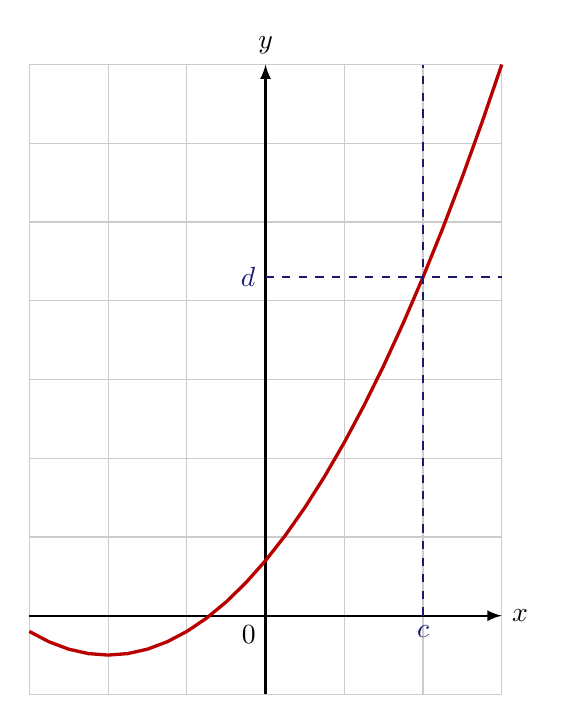
\begin{tikzpicture}
        \draw[thin,gray!40] (-3,-1) grid (3, 7);
        \draw[thick, ->, >=latex] (-3,0)--(3,0) node[right]{\(x\)};
        \draw[thick, ->, >=latex] (0,-1)--(0,7) node[above]{\(y\)};
        \draw (0, 0) node[below left] {0};

        \draw [BrickRed, very thick, domain=-3:3] plot (\x, {0.3*(\x + 2)^2 - 0.5}); 

        \draw[MidnightBlue, dashed, thick] (2, 0) node[below]{\(c\)} --(2, 7);
        \draw[MidnightBlue, dashed, thick] (0, 4.3) node[left]{\(d\)} -- (3, 4.3);
    \end{tikzpicture}
    
    \caption{As \(x\) approaches infinity, so does \(f(x)\).}
    \label{fig:Ch02-lim-inf-inf}
\end{figure}



\subsection{Handling infinities and indeterminate forms}

A limit that exists is known as a \textit{finite} limit. Finite limits can be combined in a natural way.
%
\begin{align*}
    \lim_{x \rightarrow a} (f(x) + g(x)) &= \lim_{x \rightarrow a} f(x) + \lim_{x \rightarrow a} g(x)\\
    \lim_{x \rightarrow a} (f(x) \cdot g(x)) &= \lim_{x \rightarrow a} f(x) \cdot \lim_{x \rightarrow a} g(x)\\
    \lim_{x \rightarrow a} \frac{f(x)}{g(x)} &= \frac{\lim_{x \rightarrow a} f(x)}{\lim_{x \rightarrow a} g(x)}
\end{align*}

We use the following rules to handle infinities.
%
\begin{align*}
    a \times \infty &= \infty\\
    \frac{a}{\infty} &= 0
\end{align*}

If a limit involves \(x\) approaching zero, we may sometimes have to specify the direction in which \(x\) is approaching it, i.e. whether it is approaching zero as a positive number (from the right) or as a negative number (from the left).
%
\begin{align*}
    \lim_{x \rightarrow 0^+} \frac{1}{x} &= \infty\\
    \lim_{x \rightarrow 0^-} \frac{1}{x} &= -\infty
\end{align*}

There are certain cases where we \textit{cannot} combine limits. These are called \textit{indeterminate forms}, and there is no general rule for figuring out what these indeterminate forms evaluate to. Examples of indeterminate forms are given below.
%
\[
\frac{0}{0},\; \frac{\infty}{\infty},\; 0 \times \infty,\; \infty - \infty,\; 0^0,\; 1^\infty,\; \infty^0
\]



\subsection{Little o and big O notation}

It is often useful to talk about the rate at which some function changes as its input increases (or decreases), without worrying to much about the detailed form. To do this, we introduce two types of notation: little \(o\) and big \(O\).

To compare the order of growth of two functions \(f(x)\) and \(g(x)\), we can look at the ratio of the two functions as their input approaches infinity, i.e.
%
\[\lim_{x \rightarrow \infty} \left|\frac{f(x)}{g(x)}\right|\text{.}\]
%
Let's look at how this limit behaves for different functions.


\begin{figure}[H]
    \centering

    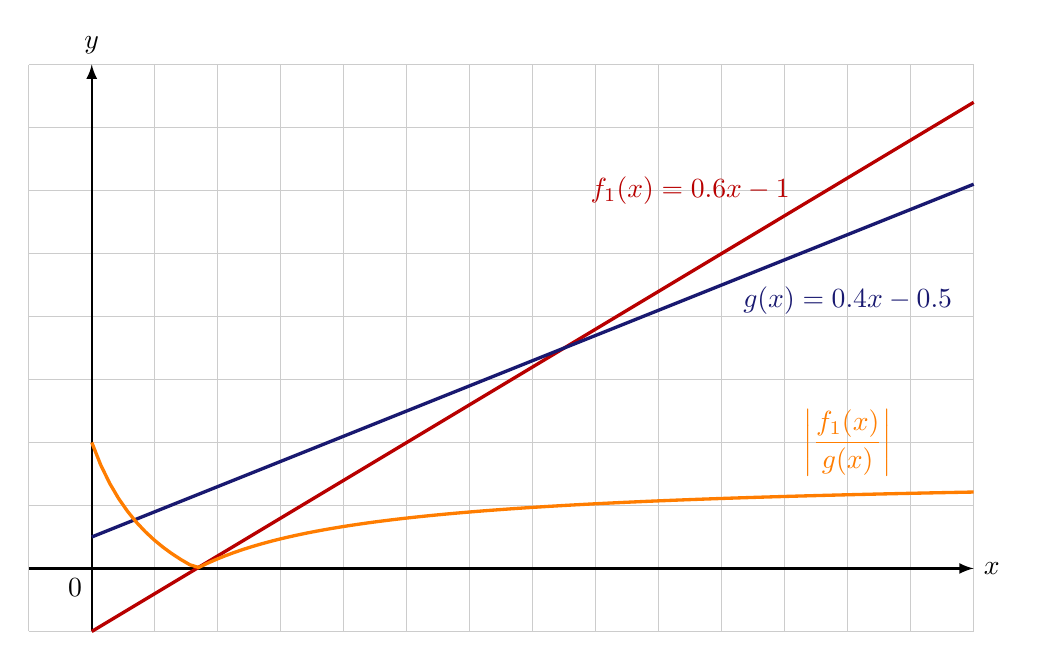
\begin{tikzpicture}[scale=0.8]
        \draw[thin,gray!40] (-1,-1) grid (14, 8);
        \draw[thick, ->, >=latex] (-1,0)--(14,0) node[right]{\(x\)};
        \draw[thick, ->, >=latex] (0,-1)--(0,8) node[above]{\(y\)};
        \draw (0, 0) node[below left] {0};

        \draw [BrickRed, very thick, domain=0:14] plot (\x, {0.6*\x-1});
        \draw node[BrickRed] at (9.5, 6) {\(f_1(x) = 0.6x - 1\)};

        \draw [MidnightBlue, very thick, domain=0:14] plot (\x, {0.4*\x+0.5});
        \draw node[MidnightBlue] at (12, 4.25) {\(g(x) = 0.4x - 0.5\)};

        \draw[BurntOrange, very thick, domain=0:14, samples=100] plot (\x, {abs((0.6*\x-1)/(0.4*\x+0.5))});
        \draw node[BurntOrange] at (12, 2) {\(\left|\dfrac{f_1(x)}{g(x)}\right|\)};
    \end{tikzpicture}
    
    \caption{Graphs of a linear function \(f_1(x)\), another linear function \(g(x)\) and the absolute value of their quotient \(|f(x)/g(x)|\).}
    \label{fig:Ch02-linear-linear-quotient-graph}
\end{figure}


Figure \ref{fig:Ch02-linear-linear-quotient-graph} shows the graphs of two functions \(f_1(x) = 0.6x - 1\) and \(g(x) = 0.4x + 0.5\). Both of these functions are linear, so they should have the same order of growth. When this happens, the limit of the ratio of the two functions, as \(x\) approaches infinity, should be a finite constant. As we see in the graph, this is indeed the case, with the orange curve converging to a value of \(1.5\).

Now consider the logarithmic function \(f_2(x) = \ln{x}\) and its relationship with \(g(x)\). As shown in figure \ref{fig:Ch02-log-linear-quotient-graph}, the limit of their ratio once again converges to a finite constant: zero. This is because the logarithmic function grows much slower than the linear function.

\begin{figure}[H]
    \centering

    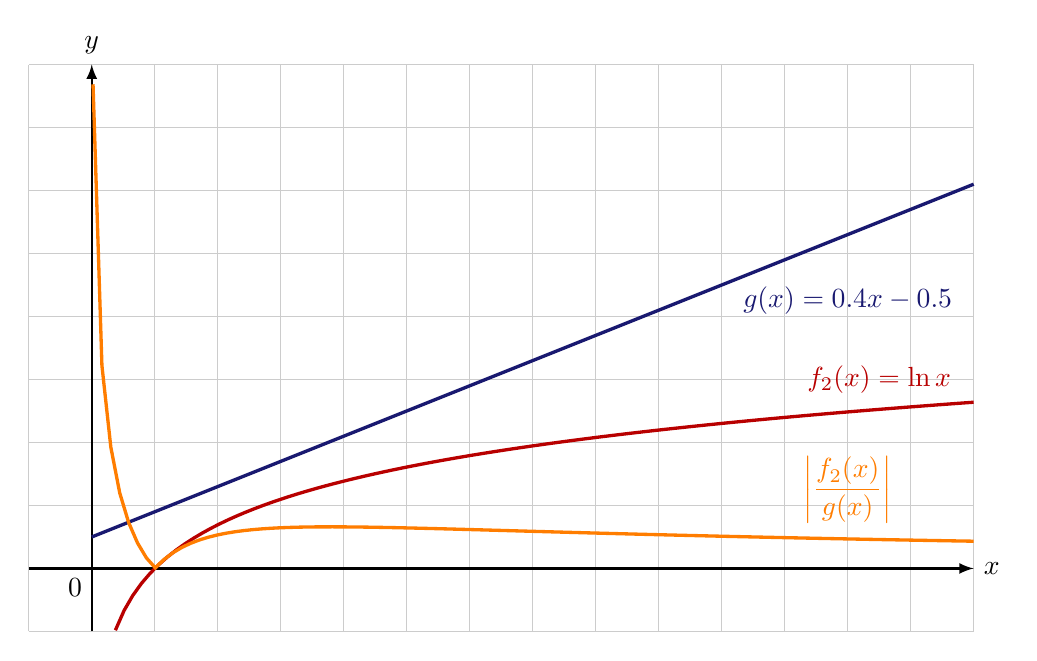
\begin{tikzpicture}[scale=0.8]
        \draw[thin,gray!40] (-1,-1) grid (14, 8);
        \draw[thick, ->, >=latex] (-1,0)--(14,0) node[right]{\(x\)};
        \draw[thick, ->, >=latex] (0,-1)--(0,8) node[above]{\(y\)};
        \draw (0, 0) node[below left] {0};

        \draw [BrickRed, very thick, domain=0.375:14, samples=100] plot (\x, {ln(\x)});
        \draw node[BrickRed] at (12.5, 3) {\(f_2(x) = \ln{x}\)};

        \draw [MidnightBlue, very thick, domain=0:14] plot (\x, {0.4*\x+0.5});
        \draw node[MidnightBlue] at (12, 4.25) {\(g(x) = 0.4x - 0.5\)};

        \draw[BurntOrange, very thick, domain=0.02:14, samples=100] plot (\x, {abs(ln(\x)/(0.4*\x+0.5))});
        \draw node[BurntOrange] at (12, 1.25) {\(\left|\dfrac{f_2(x)}{g(x)}\right|\)};
    \end{tikzpicture}
    
    \caption{Graphs of a logarithmic function \(f_2(x)\), a linear function \(g(x)\) and the absolute value of their quotient \(|f(x)/g(x)|\).}
    \label{fig:Ch02-log-linear-quotient-graph}
\end{figure}

From this we can gather that the limit of the ratio of two functions \(f(x)\) and \(g(x)\) is bounded (i.e. a finite constant) when \(f(x)\) grows \textit{as fast as} or \textit{slower} than \(g(x)\). We can denote this with big \(O\) notation, as \(f(x) = O(g(x))\). The definition of big \(O\) notation is given below.
%
\begin{quote}
    \textbf{Big \(\mathbf{O}\) notation.}

    We write \(f = O(g)\) near infinity if \(\lim_{x \rightarrow \infty} \left|\frac{f(x)}{g(x)}\right|\) is bounded, i.e.
    %
    \[\exists M \in \mathbb{R},\; \lim_{x \rightarrow \infty} \left|\frac{f(x)}{g(x)}\right| < M\text{.}\]
    
    Sometimes we want to consider the growth rate of functions not just near infinity but near a specific point \(x = b\). In this case, we write \(f = O(g)\) near \(b\) if
    %
    \[\exists M \in \mathbb{R},\; \lim_{x \rightarrow b} \left|\frac{f(x)}{g(x)}\right| < M\text{.}\]
\end{quote}

Remember that big \(O\) notation covers two cases:
%
\begin{itemize}
    \item \(f(x)\) grows as fast as \(g(x)\) (meaning that the two functions have the same order of growth), or
    \item \(f(x)\) grows slower than \(g(x\)) (meaning that the former has a lower order of growth than the latter).
\end{itemize}
%
If we want to be more specific and consider only the second case where \(f(x)\) grows strictly slower than \(g(x)\), we can use little \(o\) notation to write \(f(x) = o(g(x))\). The definition of little \(o\) notation is given below.
%
\begin{quote}
    \textbf{Little \(\mathbf{o}\) notation.}

    We write \(f = o(g)\) near infinity if \(\lim_{x \rightarrow \infty} \frac{f(x)}{g(x)} = 0\).
    
    Again, we sometimes want to consider the growth rate of functions near a specific point \(x = b\). For this we say that \(f = o(g)\) near \(b\) if \(\lim_{x \rightarrow b} \frac{f(x)}{g(x)} = 0\).    
\end{quote}

Note that since little \(o\) is a special case of big \(O\), we have \(f = o(g) \;\Rightarrow\; f = O(g)\).



\subsection{Continuity}

A function \(f\) is continuous if for all \(a\) where \(f(a)\) is defined, we have \(\lim_{x\rightarrow a} f(x) = f(a)\).

In practice, this means that the graph of \(y = f(x)\) is a single unbroken curve. The exponential and logarithm functions, for example, are both continuous.

An important result of this is the \textit{intermediate value theorem}.
%
\begin{quote}
    \textbf{Intermediate value theorem.}

    Assume for a continuous function \(f\) that \(a < b\) and \(f(a) < f(b)\). For any value \(y\) such that \(f(a) < y < f(b)\), there exists a (not necessarily unique) value \(x\) such that \(a < x < b\) and \(f(x) = y\).
\end{quote}
%
See figure \ref{fig:Ch02-int-value-thm} and \ref{fig:Ch02-int-value-thm-uniqueness}.

\begin{figure}[H]
    \centering

    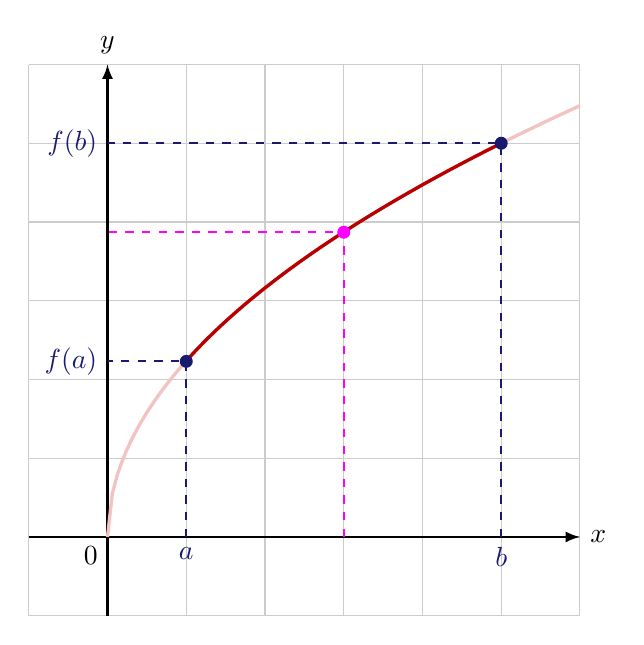
\begin{tikzpicture}
        \draw[thin,gray!40] (-1,-1) grid (6, 6);
        \draw[thick, ->, >=latex] (-1,0)--(6,0) node[right]{\(x\)};
        \draw[thick, ->, >=latex] (0,-1)--(0,6) node[above]{\(y\)};
        \draw (0, 0) node[below left] {0};

        \draw [BrickRed!20, very thick, domain=0:6, samples=100] plot (\x,
        {sqrt(5*\x)});

        \draw [BrickRed, very thick, domain=1:5, samples=100] plot (\x,
        {sqrt(5*\x)});

        \filldraw[radius=0.075, MidnightBlue] (1, 2.23) circle;
        \draw[dashed, MidnightBlue, thick] (1, 0) node[below]{\(a\)} -- (1, 2.23) -- (0, 2.23) node[left]{\(f(a)\)};

        \filldraw[radius=0.075, Fuchsia] (3, 3.87) circle;
        \draw[dashed, Fuchsia, thick] (3, 0) -- (3, 3.87) -- (0, 3.87);


        \filldraw[radius=0.075, MidnightBlue] (5, 5) circle;
        \draw[dashed, MidnightBlue, thick] (5, 0) node[below]{\(b\)} -- (5, 5) -- (0, 5) node[left]{\(f(b)\)};
    \end{tikzpicture}
    
    \caption{The intermediate value theorem.}
    \label{fig:Ch02-int-value-thm}
\end{figure}


\begin{figure}[H]
    \centering

    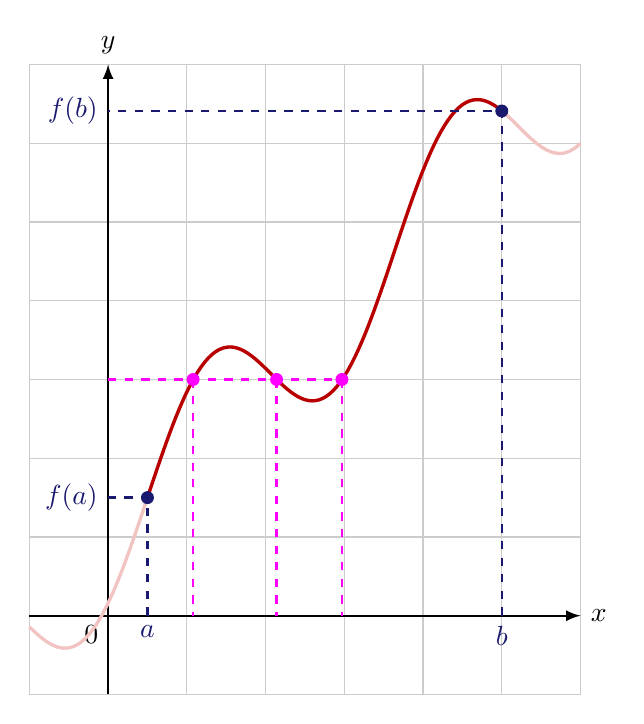
\begin{tikzpicture}
        \draw[thin,gray!40] (-1,-1) grid (6, 7);
        \draw[thick, ->, >=latex] (-1,0)--(6,0) node[right]{\(x\)};
        \draw[thick, ->, >=latex] (0,-1)--(0,7) node[above]{\(y\)};
        \draw (0, 0) node[below left] {0};

        \draw [BrickRed!20, very thick, domain=-1:6, samples=100] plot (\x,
        {sin((2*\x-1) r)+\x+1});

        \draw [BrickRed, very thick, domain=0.5:5, samples=100] plot (\x,
        {sin((2*\x-1) r)+\x+1});

        \filldraw[radius=0.075, MidnightBlue] (0.5, 1.5) circle;
        \draw[dashed, MidnightBlue, thick] (0.5, 0) node[below]{\(a\)} -- (0.5, 1.5) -- (0, 1.5) node[left]{\(f(a)\)};

        \filldraw[radius=0.075, Fuchsia] (1.08, 3) circle;
        \draw[dashed, Fuchsia, thick] (1.08, 3) -- (1.08, 0);
        \filldraw[radius=0.075, Fuchsia] (2.14, 3) circle;
        \draw[dashed, Fuchsia, thick] (2.14, 3) -- (2.14, 0);
        \filldraw[radius=0.075, Fuchsia] (2.97, 3) circle;
        \draw[dashed, Fuchsia, thick] (2.97, 3) -- (2.97, 0);

        \draw[dashed, Fuchsia, thick] (0, 3) -- (2.97, 3);

        \filldraw[radius=0.075, MidnightBlue] (5, 6.41) circle;
        \draw[dashed, MidnightBlue, thick] (5, 0) node[below]{\(b\)} -- (5, 6.41) -- (0, 6.41) node[left]{\(f(b)\)};
    \end{tikzpicture}
    
    \caption{In the intermediate value theorem, for a given value \(y\), the value of \(x\) does not necessarily have to be unique.}
    \label{fig:Ch02-int-value-thm-uniqueness}
\end{figure}

\newpage
\section{Vector spaces}

We're used to thinking of vectors as something like
%
\[\begin{bmatrix}
    3 \\ 5
\end{bmatrix}\]
%
or
%
\begin{figure}[H]
    \centering

    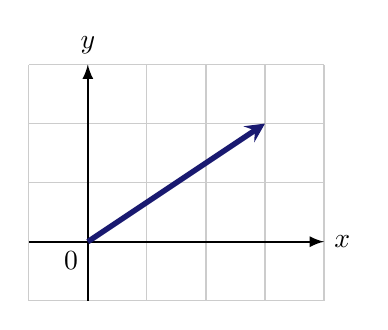
\begin{tikzpicture}[scale=0.75]
        \draw[thin,gray!40] (-1,-1) grid (4, 3);
        \draw[thick, ->, >=latex] (-1,0)--(4,0) node[right]{\(x\)};
        \draw[thick, ->, >=latex] (0,-1)--(0,3) node[above]{\(y\)};
        \draw (0, 0) node[below left] {0};
        
        \draw[line width=2pt, MidnightBlue, -stealth] (0,0)--(3,2);        
    \end{tikzpicture}
\end{figure}
%
but this is only a fraction of what the term ``vector'' encompasses. As we shall see in this section, given the correct prerequisites, even something like
%
\[
    2x^2 + 3x + 5
\]
%
can be a vector!



\subsection{What is a vector space?}

To start, we define a \textit{vector space} as follows.
%
\begin{quote}
    \textbf{Definition of a vector space.}

    For a field \(K\), a non-empty set \(V\) is a \(K\)-vector space (or a vector space over \(K\)) if, for any \(\vec{u}, \vec{v} \in V\) and any scalar \(a \in K\), we have
    %
    \begin{align*}
        \vec{u} + \vec{v} &\in V \tag{closure under vector addition}\\
        a\vec{u} &\in V \tag{closure under scalar multiplication}
    \end{align*}
    %
    The elements of \(V\) are called \textit{vectors}.
\end{quote}

We note the following:
%
\begin{itemize}
    \item Here, \(K\) is a \textit{field}, typically either \(\mathbb{R}\) or \(\mathbb{C}\). This field tells us what counts as a ``scalar'' in this vector space.
    \item The pair of properties listed in the definition give rise to what's called \textit{linearity} --- it's what makes linear algebra linear.
    \item Vector addition and scalar multiplication are governed by the following rules.
    %
    \begin{align*}
        (a + b)\vec{v} &= a\vec{v} + b\vec{v}\\
        (a(b \vec{v})) &= (ab) \vec{v}\\
        \vec{u} + \vec{v} &= \vec{v} + \vec{u}\\
        \vec{u} + (\vec{v} + \vec{w}) &= (\vec{u} + \vec{v}) + \vec{w}\\
        a(\vec{u} + \vec{v}) &= a\vec{u} + a\vec{v}\\
        \vec{v} &= \vec{v} + \vec{0}\\
        0\vec{v} &= \vec{0}\\
        1\vec{v} &= \vec{v}
    \end{align*}
    %
    where \(\vec{u}, \vec{v}, \vec{w}\) are vectors, \(a, b\) are scalars in \(K\), and \(\vec{0}\) represents the zero vector.
\end{itemize}





\subsection{Examples of vector spaces}

Based on the definition above, what counts as a vector space? (For now, let us set \(K = \mathbb{R}\) and consider only \(\mathbb{R}\)-vector spaces.)

Unsurprisingly, the set of pairs of real numbers, denoted as \(\mathbb{R}^2\), is a vector space:
%
\[
    \mathbb{R}^2 =
    \left\{
    \left.
    \begin{bmatrix}
        x \\ y
    \end{bmatrix}
    \right|
    x, y \in \mathbb{R}
    \right\}
\]
%
and each of the pairs \(\begin{bmatrix} x \\ y \end{bmatrix}\) is a vector. This is because of the fact that the sum of any two vectors in \(\mathbb{R}^2\) must also be in \(\mathbb{R}^2\), and that the scaled version of any vector in \(\mathbb{R}^2\) must also be in \(\mathbb{R}^2\). These vectors can be visualised as arrows in 2D space, as shown in figures \ref{fig:Ch03-r2-vectors-closed-under-addition} and \ref{fig:Ch03-r2-vectors-closed-under-scaling}.

\begin{figure}[H]
    \centering

    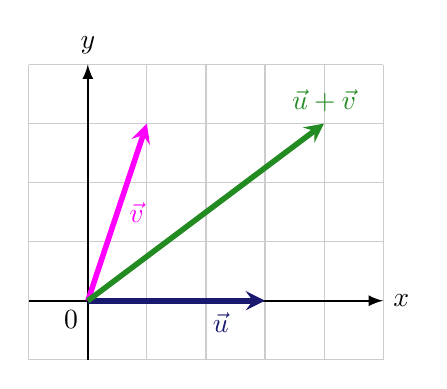
\begin{tikzpicture}[scale=0.75]
        \draw[thin,gray!40] (-1,-1) grid (5, 4);
        \draw[thick, ->, >=latex] (-1,0)--(5,0) node[right]{\(x\)};
        \draw[thick, ->, >=latex] (0,-1)--(0,4) node[above]{\(y\)};
        \draw (0, 0) node[below left] {0};
        
        \draw[line width=2pt, MidnightBlue, -stealth] (0,0)--(3,0) node[pos=3/4, below]{\(\vec{u}\)};
        
        \draw[line width=2pt, Fuchsia, -stealth] (0,0)--(1,3) node[pos=1/2, anchor=west]{\(\vec{v}\)};    
        
        \draw[line width=2pt, ForestGreen, -stealth] (0,0)--(4,3) node[above]{\(\vec{u}+\vec{v}\)};
    \end{tikzpicture}
    
    \caption{Vectors in \(\mathbb{R}^2\) are closed under addition. For any given pair of vectors \(\vec{u}\) and \(\vec{v}\) both in \(V\), their sum \(\vec{u} + \vec{v}\) must also be a vector.}
    \label{fig:Ch03-r2-vectors-closed-under-addition}
\end{figure}

\begin{figure}[H]
    \centering

    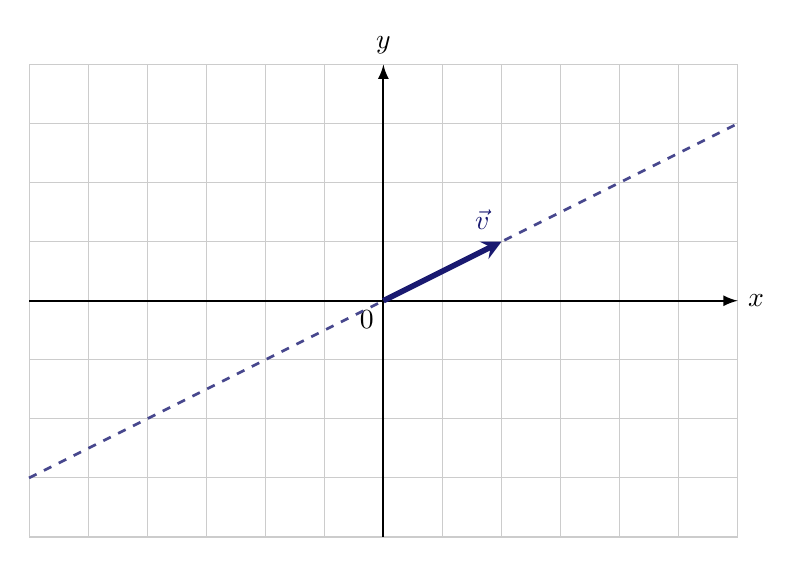
\begin{tikzpicture}[scale=0.75]
        \draw[thin,gray!40] (-6,-4) grid (6, 4);
        \draw[thick, ->, >=latex] (-6,0)--(6,0) node[right]{\(x\)};
        \draw[thick, ->, >=latex] (0,-4)--(0,4) node[above]{\(y\)};
        \draw (0, 0) node[below left] {0};

        \draw[dashed, line width=1pt, MidnightBlue!80] (-6,-3)--(6,3); 
        \draw[line width=2pt, MidnightBlue, -stealth] (0,0)--(2,1) node[above left] {\(\vec{v}\)};
         
    \end{tikzpicture}
    
    \caption{Vectors in \(\mathbb{R}^2\) are closed under scalar multiplication. For any given vector \(v \in \mathbb{R}^2\), the product between \(\vec{v}\) and any scalar \(a\) (i.e. any vector lying on the dashed line) is also a vector.}
    \label{fig:Ch03-r2-vectors-closed-under-scaling}
\end{figure}





The same goes with the set of triplets of real numbers
%
\(
\begin{bmatrix}
    x \\ y \\ z
\end{bmatrix}\),
%
which is denoted as \(\mathbb{R}^3\) and whose vectors can be visualised as arrows in 3D space. In fact, for any natural number \(n\), the set of \(n\)-tuples of real numbers (denoted as \(\mathbb{R}^n\)) is a vector space.

So far this is not very exciting as it is equivalent to our usual notion of what a ``vector'' is. To step things up a notch, let us  consider the set of polynomials of degree at most \(2\). Is this set a vector space?
%
\[
    \{ax^2 + bx + c \mid a, b, c, \in \mathbb{R}\}
\]
%
To answer this, we notice that:
%
\begin{itemize}
    \item Given any two polynomials in this set,
    %
    \begin{align*}
        \alpha &= a_1 x^2 + b_1 x + c_1\\
        \beta &= a_2 x^2 + b_2 x + c_2
    \end{align*}
    %
    their sum \(\alpha + \beta\) must also be an element of this set.

    \item If we multiply a polynomial of degree at most 2 with a scalar \(a\), the resultant product must also be a polynomial of degree at most 2.
\end{itemize}
%
This means that this set is indeed a vector space!

Table \ref{tab:Ch03-vector-space-examples} lists some examples of sets that are vector spaces, and some that aren't.

\begin{table}[H]
    \centering
    \begin{tabular}{|c|c|}
        \hline
        \textbf{Vector spaces} & \textbf{Not vector spaces}\\
        \hline
        The set of real numbers \(\mathbb{R}\) & The set of natural numbers \(\mathbb{N}\)\\
        The set of complex numbers \(\mathbb{C}\) & The set of polynomials of degree exactly 2\\
        The set of continuous functions that act on \(\mathbb{R}\) & The set of irrational numbers \(\mathbb{R} \setminus \mathbb{Q}\)\\
        \hline
    \end{tabular}
    \caption{Some sets are vector spaces while some are not.}
    \label{tab:Ch03-vector-space-examples}
\end{table}


Our previous definition of a vector space consisted of two properties. We can group those properties together to produce the following alternative but equivalent definition.
%
\begin{quote}
    \textbf{Alternative definition of a vector space.}

    For a field \(K\) (typically \(\mathbb{R}\) or \(\mathbb{C}\)), a non-empty set \(V\) is a \(K\)-vector space if, for any \(\vec{u}, \vec{v} \in V\) and any scalar \(a \in K\), we have \(a\vec{u} + \vec{v} \in V\).
\end{quote}

A vector space always contains a zero vector. This can be shown by setting \(\vec{u} = \vec{v}\) and \(a = -1\) in the definition above.




\subsection{Collinearity, span and subspaces}

Vectors \(\vec{u}\) and \(\vec{v}\) are said to be collinear if \(\vec{u} = a\vec{v}\) for some scalar \(a\). See figure \ref{fig:Ch03-collinearity}.

\begin{figure}[H]
    \centering

    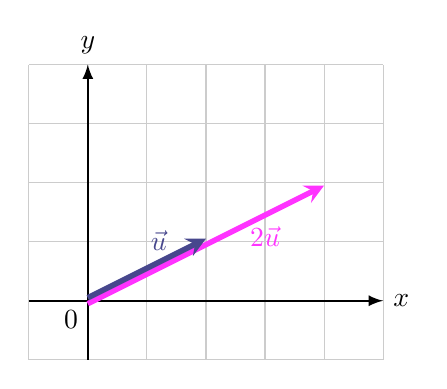
\begin{tikzpicture}[scale=0.75]
        \draw[thin,gray!40] (-1,-1) grid (5, 4);
        \draw[thick, ->, >=latex] (-1,0)--(5,0) node[right]{\(x\)};
        \draw[thick, ->, >=latex] (0,-1)--(0,4) node[above]{\(y\)};
        \draw (0, 0) node[below left] {0};
        
        \draw[line width=2pt, Fuchsia!80, -stealth, shift={(0, -0.05)}] (0,0)--(4,2) node[pos=3/4, below]{\(2\vec{u}\)};    
        \draw[line width=2pt, MidnightBlue!80, -stealth, shift={(0, 0.05)}] (0,0)--(2,1) node[pos=3/5, above]{\(\vec{u}\)};    
    \end{tikzpicture}
    
    \caption{Two collinear vectors.}
    \label{fig:Ch03-collinearity}
\end{figure}

Given some vectors \(\vec{u_1}, \vec{u_2}, \cdots, \vec{u_n}\) and some scalars \(a_1, a_2, \cdots, a_n\), the sum \(a_1 \vec{u_1} + a_2 \vec{v_2} + \cdots + a_n \vec{v_n}\) is called a \textit{linear combination} of those vectors. This is illustrated in figure \ref{fig:Ch03-linear-comb}.

\begin{figure}[H]
    \centering

    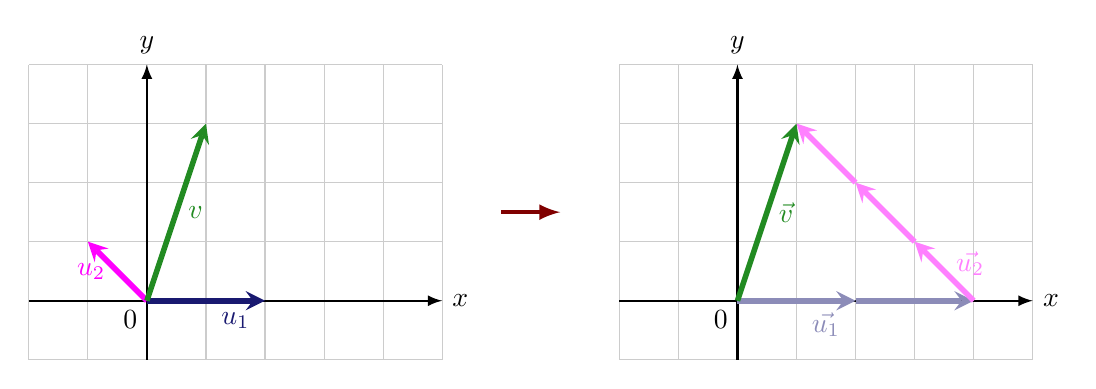
\begin{tikzpicture}[scale=0.75]
        \draw[thin,gray!40] (-2,-1) grid (5, 4);
        \draw[thick, ->, >=latex] (-2,0)--(5,0) node[right]{\(x\)};
        \draw[thick, ->, >=latex] (0,-1)--(0,4) node[above]{\(y\)};
        \draw (0, 0) node[below left] {0};
        
        \draw[line width=2pt, MidnightBlue, -stealth] (0,0)--(2,0) node[pos=3/4, below]{\(u_1\)};
        \draw[line width=2pt, Fuchsia, -stealth] (0,0)--(-1, 1) node[pos=1/2, left]{\(u_2\)};

        \draw[line width=2pt, ForestGreen, -stealth] (0,0)--(1,3) node[pos=1/2, anchor=west]{\(v\)};

        \draw[ultra thick, Maroon, ->, >=latex] (6, 1.5)--(7, 1.5);
        
        \begin{scope}[shift={(10, 0)}]
            \draw[thin,gray!40] (-2,-1) grid (5, 4);
            \draw[thick, ->, >=latex] (-2,0)--(5,0) node[right]{\(x\)};
            \draw[thick, ->, >=latex] (0,-1)--(0,4) node[above]{\(y\)};
            \draw (0, 0) node[below left] {0};
            
            \draw[line width=2pt, MidnightBlue!50, -stealth] (0,0)--(2,0) node[pos=3/4, below]{\(\vec{u_1}\)};
            \draw[line width=2pt, MidnightBlue!50, -stealth] (2,0)--(4,0);

            \draw[line width=2pt, Fuchsia!50, -stealth] (4,0)--(3, 1) node[pos=1/2, right, shift={(0, 0.1)}]{\(\vec{u_2}\)};
            \draw[line width=2pt, Fuchsia!50, -stealth] (3,1)--(2, 2);
            \draw[line width=2pt, Fuchsia!50, -stealth] (2,2)--(1, 3);

            \draw[line width=2pt, ForestGreen, -stealth] (0,0)--(1,3) node[pos=1/2, anchor=west]{\(\vec{v}\)};
        \end{scope}
        
    \end{tikzpicture}
    
    \caption{The green vector \(v\) can be expressed as a linear combination of the vectors \(u_1\) and \(u_2\), i.e. \(v = 2u_1 + 3u_2\).}
    \label{fig:Ch03-linear-comb}
\end{figure}

Given a family of vectors \(S = (\vec{u_1}, \vec{u_2}, \cdots, \vec{u_n})\), the \textit{span} of \(S\) is defined as the set of all linear combinations of the vectors in \(S\). For instance, consider the vectors shown in figure \ref{fig:Ch03-span-example}.
%
\begin{itemize}
    \item The vectors \(\vec{u}\) and \(\vec{v}\) span the \(xy\)-plane.
    \item The vectors \(\vec{u}\), \(\vec{v}\) and \(\vec{w}\) together span the entire three-dimensional space \(\mathbb{R}^3\).
    \item Since the vectors \(\vec{w}\) and \(2\vec{w}\) are collinear, their span is along a single straight line.
\end{itemize}


\tdplotsetmaincoords{60}{120}
\begin{figure}[H]
    \centering

    \begin{tikzpicture}[scale=0.75, tdplot_main_coords]
        \foreach \x in {0,1,...,5} {
            \foreach \y in {0,1,...,5} {
                \draw[thin, gray!40] (\x,-0.5) -- (\x,5.5);
                \draw[thin, gray!40] (-0.5,\y) -- (5.5,\y);
            }
        }

        \draw[thick, ->, >=latex] (0,0,0)--(5.5,0,0) node[left]{\(x\)};
        \draw[thick, ->, >=latex] (0,0,0)--(0,5.5,0) node[above]{\(y\)};
        \draw[thick, ->, >=latex] (0,0,0)--(0,0,5) node[right]{\(z\)};
        \draw (0, 0) node[above left] {0};
        
        \draw[line width=2pt, MidnightBlue, -stealth] (0,0)--(3,2) node[pos=3/4, left]{\(\vec{u}\)};
        \draw[line width=2pt, Fuchsia, -stealth] (0,0)--(1, 4) node[pos=3/4, below]{\(\vec{v}\)};
        
        \draw[line width=1pt, dashed, darkgray] (-4.5, -6, -6) -- (9, 12, 12);
        \draw[line width=2pt, ForestGreen, -stealth] (0,0,0)--(6, 8, 8) node[above]{\(2\vec{w}\)};
        \draw[line width=2pt, BurntOrange, -stealth] (0,0,0)--(3, 4, 4) node[pos=1/2, right]{\(\vec{w}\)};
    \end{tikzpicture}
    
    \caption{Three vectors in \(\mathbb{R}^3\). Both \(\vec{u}\) and \(\vec{v}\) lie flat on the \(xy\)-plane. The dashed line represents the span of \(\vec{w}\) and \(2\vec{w}\).}
    \label{fig:Ch03-span-example}
\end{figure}


Given some vector space \(V\), a subset \(U\) of \(V\) is called a \textit{subspace} if it is stable under linearity (i.e. also a vector space). For example, the \(xy\)-plane is a subspace of the three-dimensional vector space \(\mathbb{R}^3\).


\subsection{Linear independence}

The idea of \textit{linear independence} can be defined in several ways.
%
\begin{quote}
    \textbf{Definition of linear independence.}

    The vectors \(\vec{u_1},\; \vec{u_2},\; \cdots,\; \vec{u_n}\) are said to be \textit{linearly independent} if:
    %
    \begin{itemize}
        \item There exist no scalars \(a_1,\; a_2,\; \cdots,\; a_n\) (not all equal to zero) such that
        %
        \begin{equation*}\label{eq:Ch03-linear-independence}
            a_1 \vec{u_1} + a_2 \vec{u_2} + \cdots + a_n \vec{u_n} = 0 \text{.} \tag{*}
        \end{equation*}

        \item None of the vectors can be expressed as a linear combination of the others.
        
        \item None of the vectors belong to the span of the others.
    \end{itemize}
    %
    These three statements are equivalent. 
    
    To prove linear independence, we can make use of the first statement and show that for equation \eqref{eq:Ch03-linear-independence} to hold, the scalars \(a_1,\; a_2,\; \cdots,\; a_n\) must all be equal to zero.

    To disprove linear independence, we can use the second statement and show that one of the vectors can be expressed as a linear combination of the others. (Alternatively, we can provide a solution to equation \eqref{eq:Ch03-linear-independence} where not all of \(a_1,\; a_2,\; \cdots,\; a_n\) are zero.)
\end{quote}

For example, in figure \ref{fig:Ch03-span-example}, the vectors \(\vec{u}\), \(\vec{v}\) and \(\vec{w}\) are linearly independent as none of the vectors belong to the span of the others.

The example problems below demonstrate how linear independence can be proved or disproved.

\vspace{15pt}
\begin{mdframed}[linewidth=1pt]
\noindent \textbf{Problem.} Is this family of polynomials linearly independent? Explain.
%
\[\{3x,\; 4x^2 - 6x,\; 2x^2\}\] 

\textbf{Solution 1.} No. This is because one of the polynomials can be written as a linear combination of the others:
%
\[4x^2 - 6x = 2{\color{BrickRed}(2x^2)} + (-2){\color{MidnightBlue}(3x)}\]

\textbf{Solution 2.} No, because \(2{\color{MidnightBlue}(3x)} + {\color{ForestGreen}(4x^2 - 6x)} - 2{\color{BrickRed}(2x^2)}= 0\).
\vspace{10pt}
\end{mdframed}


\vspace{15pt}
\begin{mdframed}[linewidth=1pt]
\noindent \textbf{Problem.} Is this family of vectors linearly independent? Explain.
%
\[
\left\{
\begin{bmatrix}
    2 \\ 2
\end{bmatrix}
,\;
\begin{bmatrix}
    1 \\ -1
\end{bmatrix}
\right\}
\]

\textbf{Solution.} Yes. Assume there exists a linear combination such that
%
\[
a_1
\begin{bmatrix}
    2 \\ 2
\end{bmatrix}
+
a_2
\begin{bmatrix}
    1 \\ -1
\end{bmatrix}
= 0\text{.}
\]
%
This produces the following system of simultaneous equations:
%
\[
\begin{cases}
    2a_1 + a_2 = 0\\
    2a_1 - a_2 = 0
\end{cases}
\]
%
for which the only solution is \(a_1 = a_2 = 0\). Hence, the family of vectors are indeed linearly independent.
\vspace{10pt}
\end{mdframed}




\subsection{Basis}

Let \(V\) be a vector space. A basis\footnote{Plural: bases.} of \(V\) is a set \(S\) of linearly independent vectors that spans the entirety of \(V\). For instance, in figure \ref{fig:Ch03-span-example}, the set of vectors \(\{\vec{u}, \vec{v}\}\) is a basis of the \(xy\)-plane.

If the basis \(S\) is finite, then the size (cardinality) of \(S\) is referred to as the \textit{dimension} of \(V\). This means that the \(xy\)-plane in figure \ref{fig:Ch03-span-example} has a dimension of \(2\).

One of the most obvious bases for \(\mathbb{R}^n\) is
%
\[
\left\{
\begin{bmatrix}
    1 \\ 0 \\ 0 \\ \vdots \\ 0
\end{bmatrix},\;
%
\begin{bmatrix}
    0 \\ 1 \\ 0 \\ \vdots \\ 0
\end{bmatrix},\;
%
\begin{bmatrix}
    0 \\ 0 \\ 1 \\ \vdots \\ 0
\end{bmatrix},\;
%
\cdots,\;
%
\begin{bmatrix}
    0 \\ 0 \\ 0 \\ \vdots \\ 1
\end{bmatrix}
\right\}
\]
%
which is known as the \textit{canonical basis}. See figures \ref{fig:Ch03-canonical-basis-2d} and \ref{fig:Ch03-canonical-basis-3d}.

\begin{figure}[H]
    \centering

    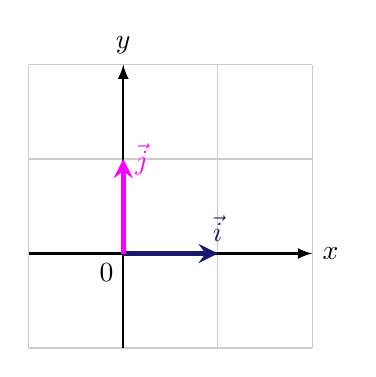
\begin{tikzpicture}[scale=1.2]
        \draw[thin,gray!40] (-1,-1) grid (2, 2);
        \draw[thick, ->, >=latex] (-1,0)--(2,0) node[right]{\(x\)};
        \draw[thick, ->, >=latex] (0,-1)--(0,2) node[above]{\(y\)};
        \draw (0, 0) node[below left] {0};
        
        \draw[line width=2pt, MidnightBlue, -stealth] (0,0)--(1,0) node[above]{\(\vec{i}\)};  
        \draw[line width=2pt, Fuchsia, -stealth] (0,0)--(0,1) node[right]{\(\vec{j}\)};
    \end{tikzpicture}
    
    \caption{The canonical basis \(\{\vec{i}, \vec{j}\}\) of \(\mathbb{R}^2\).}
    \label{fig:Ch03-canonical-basis-2d}
\end{figure}



\tdplotsetmaincoords{60}{120}
\begin{figure}[H]
    \centering

    \begin{tikzpicture}[scale=1.2, tdplot_main_coords]
        \foreach \x in {0,1,2} {
            \foreach \y in {0,1,2} {
                \draw[thin, gray!40] (\x,-0.5) -- (\x,2.5);
                \draw[thin, gray!40] (-0.5,\y) -- (2.5,\y);
            }
        }

        \draw[thick, ->, >=latex] (0,0,0)--(2.5,0,0) node[left]{\(x\)};
        \draw[thick, ->, >=latex] (0,0,0)--(0,2.5,0) node[above]{\(y\)};
        \draw[thick, ->, >=latex] (0,0,0)--(0,0,2.5) node[right]{\(z\)};
        \draw (0, 0) node[above left] {0};
        
        \draw[line width=2pt, MidnightBlue, -stealth] (0,0)--(1,0) node[pos=3/4, above left]{\(\vec{i}\)};
        \draw[line width=2pt, Fuchsia, -stealth] (0,0)--(0, 1) node[pos=3/4, above]{\(\vec{j}\)};
        \draw[line width=2pt, BurntOrange, -stealth] (0,0,0)--(0, 0, 1) node[above right]{\(\vec{k}\)};
    \end{tikzpicture}
    
    \caption{The canonical basis \(\{\vec{i}, \vec{j}, \vec{k}\}\) of \(\mathbb{R}^3\).}
    \label{fig:Ch03-canonical-basis-3d}
\end{figure}





\subsection{Linear maps}

We define a \textit{linear map} or \textit{linear mapping} as follows.
%
\begin{quote}
    \textbf{Definition of a linear map.}

    For two \(K\)-vector spaces \(V\) and \(W\), consider a function \(f : V \to W\) that maps each vector in \(V\) to a vector in \(W\).
    
    This function is said to be a \textit{linear map} if, for any two vectors \(\vec{u}, \vec{v} \in V\) and any scalar \(a \in K\), we have
    %
    \begin{align*}
        f(\vec{u} + \vec{v}) &= f(\vec{u}) + f(\vec{v})\\
        f(a\vec{u}) &= a f(\vec{u})\text{.}
    \end{align*}
\end{quote}

Once again we can combine the two equations above to get an alternative but equivalent definition.
%
\begin{quote}
    \textbf{Alternative definition of a linear map.}
    
    The function \(f : V \to W\) is said to be a \textit{linear map} if, for any two vectors \(\vec{u}, \vec{v} \in V\) and any scalar \(a \in K\), we have \(f(a\vec{u} + \vec{v}) = a f(\vec{u}) + f(\vec{v})\).
\end{quote}
%
For any linear map \(f\) we must have \(f(\vec{0}) = \vec{0}\). This can be shown by setting \(a = 0\) and \(\vec{v} = \vec{0}\) in the definition above.

An example of a linear map in \(\mathbb{R}^2\) is a function \(f\) that rotates vectors by \(90\degree\) anticlockwise, i.e.
%
\[
f\left(
    \begin{bmatrix}
        x \\ y
    \end{bmatrix}
\right)
=
\begin{bmatrix}
    -y \\ x
\end{bmatrix}
\]
%
To prove this, consider any two vectors \(\vec{u} = \begin{bmatrix} x_1 \\ y_1 \end{bmatrix}\) and \(\vec{v} = \begin{bmatrix} x_2 \\ y_2 \end{bmatrix}\). For any scalar \(a \in \mathbb{R}\), we have
%
\begin{align*}
    f(a\vec{u} + \vec{v}) &= f\left(a \begin{bmatrix} x_1 \\ y_1 \end{bmatrix} + \begin{bmatrix} x_2 \\ y_2 \end{bmatrix}\right)\\
    &= f\left(\begin{bmatrix} ax_1 \\ ay_1 \end{bmatrix} + \begin{bmatrix} x_2 \\ y_2 \end{bmatrix}\right)\\
    &= f\left(\begin{bmatrix} ax_1 + x_2 \\ ay_1 + y_2\end{bmatrix}\right)\\
    &= \begin{bmatrix} - ay_1 - y_2\\ ax_1 + x_2\end{bmatrix}\\
    &= \begin{bmatrix} - ay_1\\ ax_1\end{bmatrix} + \begin{bmatrix} - y_2\\ x_2\end{bmatrix}\\
    &= a \begin{bmatrix} - y_1\\ x_1\end{bmatrix} + \begin{bmatrix} - y_2\\ x_2\end{bmatrix}\\
    &= a f\left(\begin{bmatrix} x_1 \\ y_1 \end{bmatrix}\right) + f\left(\begin{bmatrix} x_2 \\ y _ 2 \end{bmatrix}\right)\\
    &= a f(\vec{u}) + f(\vec{v})
\end{align*}
%
which shows that \(f\) is a linear map. In fact, rotations, scalings and projections are all examples of linear maps in \(\mathbb{R}^2\).

If a linear map maps vectors from a vector space to the same vector space, i.e.
%
\[f: V \to V\]
%
then this mapping is known as an \textit{endomorphism}\footnote{From ``endo-'' (meaning ``internal'' in Greek) and ``morphism'' (a mathematical term for structure-preserving mappings).}. For instance, the \(90\degree\) rotation function we saw before maps vectors in \(\mathbb{R}^2\) to vectors in \(\mathbb{R}^2\), so it is an endomorphism.

Let \(U\), \(V\) and \(W\) be vector spaces. Given two linear maps:
%
\begin{align*}
    f: U &\to V\\
    g: V &\to W
\end{align*}
%
we can \textit{compose} them into a new linear map
%
\[g \circ f : U \to W\]
%
where \(f\) is applied first, then \(g\).





\subsection{Kernel and image}

Consider the linear map \(f : V \to W\), where \(V\) and \(W\) are vector spaces. We define the following:
%
\begin{itemize}
    \item The \textit{kernel} of \(f\), denoted as \(\kernel(f)\), is the set of vectors \(v \in V\) for which \(f(v) = \vec{0}\).
    \item The \textit{image} of \(f\), denoted as \(\image(f)\), is the set of \(f(v)\) for every \(v \in V\).
\end{itemize}
%
Both \(\kernel(f)\) and \(image(f)\) are vector spaces. Note that \(\kernel(f)\) always contains \(\vec{0}\) since \(f(\vec{0}) = \vec{0}\).

As an example, consider the following linear map.
%
\[
g\left(
    \begin{bmatrix}
        x \\ y
    \end{bmatrix}
\right)
=
\begin{bmatrix}
    x + y\\
    x + y
\end{bmatrix}
\]

To find its kernel \(\kernel(g)\), we solve
%
\begin{align*}
    g\left(
        \begin{bmatrix}
            x \\ y
        \end{bmatrix}
    \right)
    &= \vec{0} \\
    %
    \begin{bmatrix}
        x + y\\
        x + y
    \end{bmatrix}
    &=
    \begin{bmatrix}
        0\\
        0
    \end{bmatrix}\\
    %
    x + y &= 0\\
    y &= -x
\end{align*}
%
which gives us
%
\[
\kernel(g) =
%
\left\{\left.
    \begin{bmatrix}
        x \\ -x
    \end{bmatrix}
    \right|
    x \in \mathbb{R}
\right\}
%
= \Span\left(
    \begin{bmatrix}
        1 \\ -1
    \end{bmatrix}
\right)
\text{.}
\]

To find the image \(\image(g)\), we want to look for vectors \(\vec{v}\) that verify \(g(\vec{u}) = \vec{v}\) for some \(\vec{u}\). To do this, it might be useful to look at some examples and search for patterns.
%
\begin{align*}
    g\left(
        \begin{bmatrix}
            1 \\ 2
        \end{bmatrix}
    \right)
    &= \begin{bmatrix}
        3 \\ 3
    \end{bmatrix} \\
    g\left(
        \begin{bmatrix}
            3 \\ 4
        \end{bmatrix}
    \right)
    &= \begin{bmatrix}
        7 \\ 7
    \end{bmatrix} \\
    g\left(
        \begin{bmatrix}
            -5 \\ 3
        \end{bmatrix}
    \right)
    &= \begin{bmatrix}
        -2 \\ -2
    \end{bmatrix}
\end{align*}
%
We notice that the entries in the output vectors are always identical. We formalise this as follows --- for \(\vec{v} = g(\vec{u})\) to be true, we must have
%
\begin{align*}
    \exists x, y,\; \vec{v} &= \begin{bmatrix} x + y \\ x + y \end{bmatrix}\\
    \exists z,\; \vec{v} &= \begin{bmatrix} z \\ z \end{bmatrix}
\end{align*}
%
which yields \(\image(g) = \Span\left(\begin{bmatrix} 1 \\ 1 \end{bmatrix}\right)\).



\newpage
\section{Matrices}

A vector can be multiplied by a matrix as follows.
%
\[
\begin{bmatrix}
    a & b\\
    c & d
\end{bmatrix}
\begin{bmatrix}
    x \\ y
\end{bmatrix}
=
\begin{bmatrix}
    ax + by\\
    cx + dy
\end{bmatrix}
\]

Figure \ref{fig:Ch04-matrix-vector-mult} shows a diagrammatic representation of this procedure.

\begin{figure}[H]
    \centering

    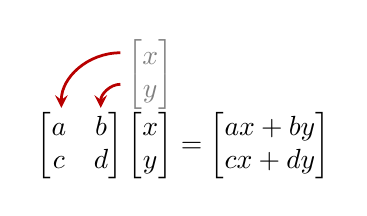
\begin{tikzpicture}[scale=1]
        \node at (0,0) {\(
            \begin{bmatrix}
                a & b\\
                c & d
            \end{bmatrix}
            \overset{{\color{gray}
                \begin{bmatrix}
                    x \\ y
                \end{bmatrix}
            }}{
                \begin{bmatrix}
                    x \\ y
                \end{bmatrix}
            }
            =
            \begin{bmatrix}
                ax + by\\
                cx + dy
            \end{bmatrix}
        \)};

        \draw[line width=1pt, -stealth, BrickRed] (-0.8, 0.7) arc (90:180:0.75 and 0.7);
        \draw[line width=1pt, -stealth, BrickRed] (-0.8, 0.3) arc (90:180:0.25 and 0.3);
    \end{tikzpicture}
    
    \caption{Multiplying a matrix by a vector.}
    \label{fig:Ch04-matrix-vector-mult}
\end{figure}

Notice how a matrix maps a vector, \(\begin{bmatrix} x \\ y \end{bmatrix}\), to a new one, \(\begin{bmatrix} ax + by\\ cx + dy \end{bmatrix}\), just like a linear map does. This is not a coincidence --- it is in fact possible to express any linear map as a matrix, as we shall see below.





\subsection{Expressing linear maps as matrices}

Consider two vector spaces:
%
\begin{itemize}
    \item A vector space \(U\) of \(n\) dimensions, with a specified set of basis vectors.
    \item A vector space \(V\) of \(m\) dimensions, with a specified set of basis vectors.
\end{itemize}
%
Every linear map \(f : U \to V\) can then be represented by a matrix \(M\) with \(m\) rows and \(n\) columns. Each column represents the image of a basis vector of \(U\), expressed in the basis of \(V\).

It's important to take a moment to digest what this means. Several examples are included below.



\subsubsection{Example 1: An endomorphism with unchanged bases}

\vspace{15pt}
\begin{mdframed}[linewidth=1pt]
\noindent \textbf{Setup.} We set both \(U\) and \(V\) to \(\mathbb{R}^2\). We will use the canonical basis for both vector spaces:
%
\[
\left\{
    \begin{bmatrix}
        1 \\ 0
    \end{bmatrix},
    \begin{bmatrix}
        0 \\ 1
    \end{bmatrix}
\right\}\text{.}
\]

We define \(f\) to be a linear map that scales the length of a vector by a factor of \(1.5\) and then rotates it by \(30\degree\). See figure \ref{fig:Ch04-example-1}.

We want to find the matrix \(M\) that represents this endomorphism.

\begin{figure}[H]
    \centering

    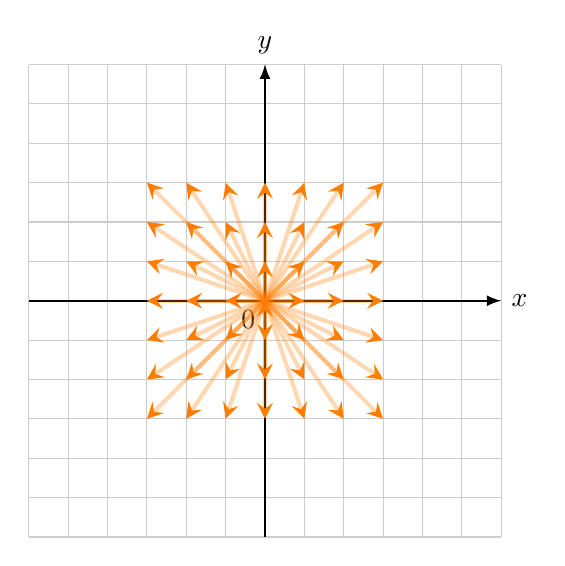
\begin{tikzpicture}[scale=0.5]
        \draw[thin,gray!40] (-6,-6) grid (6, 6);
        \draw[thick, ->, >=latex] (-6,0)--(6,0) node[right]{\(x\)};
        \draw[thick, ->, >=latex] (0,-6)--(0,6) node[above]{\(y\)};
        \draw (0, 0) node[below left] {0};
        
        \foreach \x in {-3,...,3} {
            \foreach \y in {-3,...,3} {
                \draw[line width=1.5pt, BurntOrange, -stealth, draw opacity=0.3] (0,0)--(\x,\y);
            }
        }
    \end{tikzpicture}

    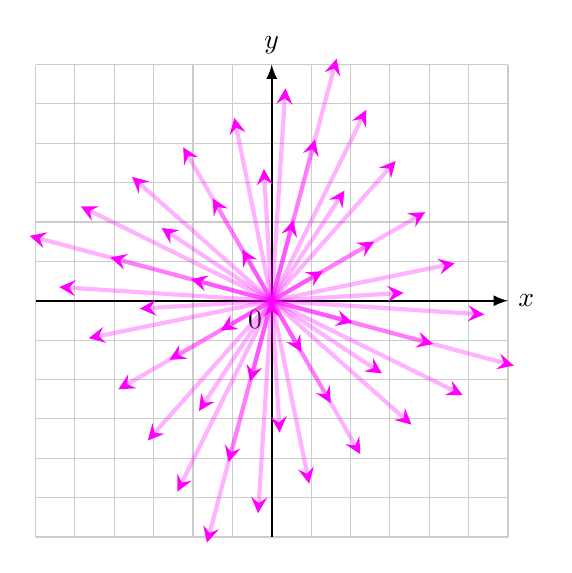
\begin{tikzpicture}[scale=0.5]
        \draw[thin,gray!40] (-6,-6) grid (6, 6);
        \draw[thick, ->, >=latex] (-6,0)--(6,0) node[right]{\(x\)};
        \draw[thick, ->, >=latex] (0,-6)--(0,6) node[above]{\(y\)};
        \draw (0, 0) node[below left] {0};
        
        \foreach \x in {-3,...,3} {
            \foreach \y in {-3,...,3} {
                \draw[line width=1.5pt, Fuchsia, -stealth, draw opacity=0.3] (0,0) -- ($1.5*({cos(30) * \x + cos(120) * \y}, {sin(30) * \x + sin(120) * \y})$);
            }
        }
    \end{tikzpicture}
    
    \caption{The linear map \(f\) takes a vector (in orange) and scales it by a factor of \(1.5\) before rotating it by \(30\degree\) anticlockwise. This results in a new vector (in purple).}
    \label{fig:Ch04-example-1}
\end{figure}

\vspace{2pt}
\end{mdframed}


Let's start with the size of the matrix, also known as its \textit{order}. We know both \(U\) and \(V\) are 2-dimensional vector spaces, so the matrix is going to have an order of \(2 \times 2\), with two rows and two columns.
%
\[
M = \begin{bmatrix}
    \color{BrickRed}\square & \color{MidnightBlue}\square\\
    \color{BrickRed}\square & \color{MidnightBlue}\square\\
\end{bmatrix}
\]

Remember that each column of the matrix represents the image of a basis vector of \(U\), expressed in the basis of \(V\). This means that the first column (in red) will represent where the first basis vector of \(U\) will get mapped to, as expressed using the basis vectors of \(V\).
%
\begin{itemize}
    \item The first basis vector of \(U\) is \(\begin{bmatrix} 1 \\ 0 \end{bmatrix}\). Following the rule of our transformation, the linear map will take us to \(\begin{bmatrix} 2\cos{30\degree} \\ 2\sin{30\degree} \end{bmatrix}\). Since the bases are the same for both vector spaces, this will be the first column of our matrix \(M\).
    \item Similarly, the second basis vector of \(U\) is \(\begin{bmatrix} 0 \\ 1 \end{bmatrix}\). This maps to \(\begin{bmatrix} 2\cos{120\degree} \\ 2\sin{120\degree} \end{bmatrix}\), or \(\begin{bmatrix} -2\sin{30\degree} \\ 2\cos{30\degree} \end{bmatrix}\). Again, the bases are the same for both vector spaces, so this will be the second column of our matrix \(M\).
\end{itemize}
%
Hence, the linear map \(f\) is represented by the matrix
%
\[
M = \begin{bmatrix}
    2\cos{30\degree} & -2\sin{30\degree}\\
    2\sin{30\degree} & 2\cos{30\degree}
\end{bmatrix}
%
= \begin{bmatrix}
    \sqrt{3} & -1\\
    1 & \sqrt{3}
\end{bmatrix}
\]
%
and this matrix can be applied to any vector in \(U\). For instance, consider the input vector \(\vec{v} = \begin{bmatrix} 3 \\ 2 \end{bmatrix}\). To find out what this vector maps to, we simply work out the following expression:
%
\begin{align*}
    M\vec{v} &= \begin{bmatrix}
        \sqrt{3} & -1\\
        1 & \sqrt{3}
    \end{bmatrix}
    \begin{bmatrix} 3 \\ 2 \end{bmatrix}\\
    %
    &= \begin{bmatrix}
        3\sqrt{3} - 2\\
        2\sqrt{3} + 3
    \end{bmatrix}
\end{align*}
%
to get our answer. This is verified in figure \ref{fig:Ch04-example-1-verification}.

\begin{figure}[H]
    \centering

    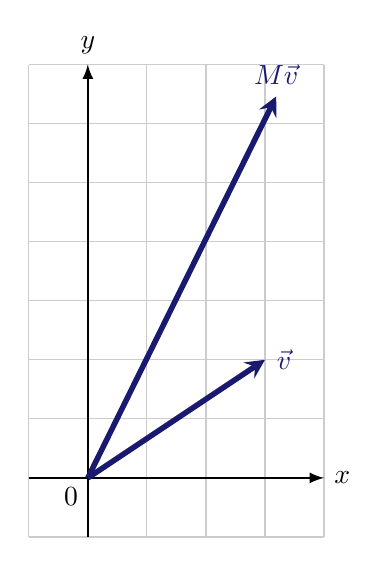
\begin{tikzpicture}[scale=0.75]
        \draw[thin,gray!40] (-1,-1) grid (4, 7);
        \draw[thick, ->, >=latex] (-1,0)--(4,0) node[right]{\(x\)};
        \draw[thick, ->, >=latex] (0,-1)--(0,7) node[above]{\(y\)};
        \draw (0, 0) node[below left] {0};
        
        \draw[line width=2pt, MidnightBlue, -stealth] (0,0)--(3,2) node[right]{\(\vec{v}\)};
        \draw[line width=2pt, MidnightBlue, -stealth] (0,0)--(1.73*3-2, 1.73*2+3) node[above]{\(M\vec{v}\)};
    \end{tikzpicture}
    
    \caption{Verifying the equivalence between the linear map \(f\) and the matrix \(M = \begin{bmatrix} \sqrt{3} & -1 \\ 1 & \sqrt{3} \end{bmatrix}\) by using an example vector \(\vec{v} = \begin{bmatrix} 3 \\ 2 \end{bmatrix}\).}
    \label{fig:Ch04-example-1-verification}
\end{figure}




\subsubsection{Example 2: An endomorphism with changed bases}

\vspace{15pt}
\begin{mdframed}[linewidth=1pt]
\noindent \textbf{Setup.} Like the previous example, we set both \(U\) and \(V\) to \(\mathbb{R}^2\), and we want to find a matrix \(M\) that corresponds to a linear map \(f\) where vectors are scaled 1.5 times and rotated by \(30\degree\) anticlockwise.

Only this time, we will use the canonical basis for the vector space \(U\):
%
\[
\left\{
    \begin{bmatrix}
        1 \\ 0
    \end{bmatrix},
    \begin{bmatrix}
        0 \\ 1
    \end{bmatrix}
\right\}
\]
%
and the following basis for \(V\). (Note that this is a basis since the two vectors are linearly independent.)
%
\[
\left\{
    \begin{bmatrix}
        2 \\ 0
    \end{bmatrix},
    \begin{bmatrix}
        -1 \\ 1
    \end{bmatrix}
\right\}
\]

\vspace{2pt}
\end{mdframed}


The process is really the same. We know from the previous example that the canonical basis vectors will be mapped to \(\begin{bmatrix} \sqrt{3} \\ 1 \end{bmatrix}\) and \(\begin{bmatrix} -1 \\ \sqrt{3} \end{bmatrix}\) respectively. All we have to do now is to express these vectors using the basis of \(V\).

Let's take the first vector \(\begin{bmatrix} \sqrt{3} \\ 1 \end{bmatrix}\) as an example. We want to find scalars \(x_1\) and \(y_1\) such that
%
\[x_1 \begin{bmatrix} 2 \\ 0 \end{bmatrix} + y_1 \begin{bmatrix} -1 \\ 1 \end{bmatrix} = \begin{bmatrix} \sqrt{3} \\ 1 \end{bmatrix}\text{.}\]
%
This has the solution of \(x_1 = (\sqrt{3}+1)/2\) and \(y_1 = 1\). In other words, the image of our first basis vector can be expressed using the basis of \(V\) as \(\begin{bmatrix} (\sqrt{3}+1)/2 \\ 1 \end{bmatrix}\). This will be the first column of our matrix \(M\).

Similarly, we want to find scalars \(x_2\) and \(y_2\) such that
%
\[x_2 \begin{bmatrix} 2 \\ 0 \end{bmatrix} + y_2 \begin{bmatrix} -1 \\ 1 \end{bmatrix} = \begin{bmatrix} -1 \\ \sqrt{3} \end{bmatrix}\text{.}\]
%
This has the solution of \(x_2 = (\sqrt{3}-1)/2\) and \(y_2 = \sqrt{3}\). This gives us the second column of our matrix: \(\begin{bmatrix} (\sqrt{3}-1)/2 \\ \sqrt{3} \end{bmatrix}\).

Hence, the matrix that is equivalent to \(f\) is given by
%
\[
M = 
\begin{bmatrix}
    (\sqrt{3}+1)/2 & (\sqrt{3}-1)/2\\
    1 & \sqrt{3}
\end{bmatrix}\text{.}
\]

Comparing this to the previous example, we see that the same linear map can be represented as different matrices depending on the chosen bases.




\subsubsection{Example 3: Non-endomorphism}

\vspace{15pt}
\begin{mdframed}[linewidth=1pt]
\noindent \textbf{Setup.} Now for something a bit different. Let us set \(U = \mathbb{R}^3\) and \(V = \mathbb{R}^2\).

Define \(f\) as the linear map that projects a vector onto the \(xy\)-plane. In other words, the linear map takes some vector \(\vec{v}\) in three-dimensional space, casts its shadow onto the \(xy\)-plane, and returns a vector that represents that shadow. See figure \ref{fig:Ch04-example-3}.

We will use the canonical bases for both \(U\) and \(V\), i.e.
%
\[
\left\{
    \begin{bmatrix}
        1 \\ 0 \\ 0
    \end{bmatrix},
    \begin{bmatrix}
        0 \\ 1 \\ 0
    \end{bmatrix},
    \begin{bmatrix}
        0 \\ 0 \\ 1
    \end{bmatrix}
\right\}
\]
%
and
%
\[
\left\{
    \begin{bmatrix}
        1 \\ 0
    \end{bmatrix},
    \begin{bmatrix}
        0 \\ 1
    \end{bmatrix}
\right\}
\]
respectively.

We want to find a matrix \(M\) that represents this linear map.

\begin{figure}[H]
    \centering

    \begin{tikzpicture}[scale=0.75, tdplot_main_coords]
        \foreach \x in {0,...,4} {
            \foreach \y in {0,...,4} {
                \draw[thin, gray!40] (\x,-0.5) -- (\x,4.5);
                \draw[thin, gray!40] (-0.5,\y) -- (4.5,\y);
            }
        }

        \draw[thick, ->, >=latex] (0,0,0)--(4,0,0) node[left]{\(x\)};
        \draw[thick, ->, >=latex] (0,0,0)--(0,4,0) node[above]{\(y\)};
        \draw[thick, ->, >=latex] (0,0,0)--(0,0,4) node[right]{\(z\)};
        \draw (0, 0) node[above left] {0};
        
        \foreach \x in {0,...,3} {
            \foreach \y in {0,...,3} {
                \foreach \z in {0,...,3} {
                    \draw[line width=1.5pt, BurntOrange, -stealth, draw opacity=0.3] (0,0,0)--(\x, \y, \z);
                }
            }
        }
    \end{tikzpicture}

    \begin{tikzpicture}[scale=0.75, tdplot_main_coords]
        \foreach \x in {0,...,4} {
            \foreach \y in {0,...,4} {
                \draw[thin, gray!40] (\x,-0.5) -- (\x,4.5);
                \draw[thin, gray!40] (-0.5,\y) -- (4.5,\y);
            }
        }

        \draw[thick, ->, >=latex] (0,0,0)--(4,0,0) node[left]{\(x\)};
        \draw[thick, ->, >=latex] (0,0,0)--(0,4,0) node[above]{\(y\)};
        \draw (0, 0) node[above left] {0};
        
        \foreach \x in {0,...,3} {
            \foreach \y in {0,...,3} {
                \draw[line width=1.5pt, Fuchsia, -stealth] (0,0,0)--(\x, \y, 0);
            }
        }
    \end{tikzpicture}
    
    \caption{The linear map \(f\) projects a three-dimensional vector (in orange) onto the \(xy\)-plane. This results in a new two-dimensional vector (in purple).}
    \label{fig:Ch04-example-3}
\end{figure}

\vspace{2pt}
\end{mdframed}

Firstly, we note that since we are mapping from a three-dimensional vector space to a two-dimensional one, our matrix must have the order \(3 \times 2\) with three rows and two columns.
%
\[
M = \begin{bmatrix}
    \color{BrickRed}\square & \color{MidnightBlue}\square & \color{OliveGreen}\square\\
    \color{BrickRed}\square & \color{MidnightBlue}\square & \color{OliveGreen}\square\\
\end{bmatrix}
\]
%
Again, each column of the matrix represents the image of a basis vector of \(U\), expressed in the basis of \(V\). Following this principle:
%
\begin{itemize}
    \item The first basis vector of \(U\) is \(\begin{bmatrix} 1 \\ 0 \\ 0 \end{bmatrix}\). Its projection is \(\begin{bmatrix} 1 \\ 0 \end{bmatrix}\).
    \item The second basis vector is \(\begin{bmatrix} 0 \\ 1 \\ 0 \end{bmatrix}\), which has the projection \(\begin{bmatrix} 0 \\ 1 \end{bmatrix}\).
    \item The third basis vector is \(\begin{bmatrix} 0 \\ 0 \\ 1 \end{bmatrix}\), with the projection \(\begin{bmatrix} 0 \\ 0 \end{bmatrix}\).
\end{itemize}
%
We're basically just losing the \(z\)-coordinate. Each of these projections is a column in our matrix \(M\). This yields
%
\[
M = \begin{bmatrix}
    1 & 0 & 0\\
    0 & 1 & 0
\end{bmatrix}
\]
which is equivalent to the linear map \(f\).




\subsubsection{Kernels and images}

Given a linear map \(f\) and its equivalent matrix \(M\), we have the following.
%
\begin{align*}
    \kernel(M) &= \kernel(f)\\
    \image(M) &= \image(f)
\end{align*}




\subsection{The elements of a matrix}

The numbers inside a matrix are called \textit{elements} or \textit{coefficients}. A matrix of order \(m \times n\) can be indexed in the following manner.
%
\[
A =
\begin{bmatrix}
    a_{1,1} & a_{1,2} & \cdots & a_{1,n}\\
    a_{2,1} & a_{2,2} & \cdots & a_{2,n}\\
    \vdots & \vdots & \ddots & \vdots\\
    a_{m,1} & a_{m,2} & \cdots & a_{m,n}
\end{bmatrix}
\]
%
Here, the element in the \(i\)-th row and \(j\)-th column is denoted as \(a_{i,j}\).



\subsection{Matrix arithmetic}

Let \(\mathcal{M}_{m, n}(\mathbb{R})\) denote the set of matrices with \(m\) rows and \(n\) columns containing real coefficients.

These matrices can be added or subtracted element-by-element.
%
\begin{align*}
    M + Q &= 
    \begin{bmatrix}
        &&\\
        & m_{i,j} + q_{i,j} & \\
        &&
    \end{bmatrix}\\
    %
    M - Q &= 
    \begin{bmatrix}
        &&\\
        & m_{i,j} - q_{i,j} & \\
        &&
    \end{bmatrix}\\
\end{align*}

They can also be multiplied by a scalar.
%
\[
aM = 
\begin{bmatrix}
    &&\\
    & a \cdot m_{i,j} & \\
    &&
\end{bmatrix}
\]

Notice that the order of matrices do not change when they are added or multiplied. This means that \(\mathcal{M}_{m, n}(\mathbb{R})\) is itself a vector space.

Moreover, matrices can also be multiplied, but only if their sizes match. The product of two matrices \(MQ\) is only valid when
%
\begin{align*}
    M &\in \mathcal{M}_{m, {\color{BrickRed} n}}(\mathbb{R})\\
    Q &\in \mathcal{M}_{{\color{BrickRed} n}, k}(\mathbb{R})\\
\end{align*}
%
for some integers \(m\), \(n\) and \(k\). See figure \ref{fig:Ch04-matrix-mult-restraint}.


\begin{figure}[H]
    \centering

    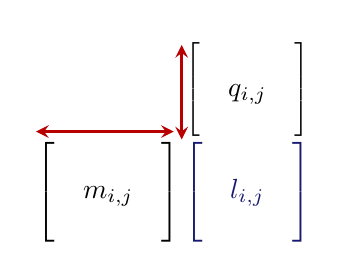
\begin{tikzpicture}[scale=1]
        \node at (0,0) {\(
            \begin{bmatrix}
                &&\\
                & m_{i,j} &\\
                &&
            \end{bmatrix}
            \overset{
                \begin{bmatrix}
                    &&\\
                    & q_{i,j} &\\
                    &&
                \end{bmatrix}
            }{{\color{MidnightBlue}
                \begin{bmatrix}
                    &&\\
                    & l_{i,j} &\\
                    &&
                \end{bmatrix}
            }}
        \)};

        \draw[line width=1pt, stealth-stealth, BrickRed, shift={(0.1, 0)}] (0,0) -- (0,1.2);
        \draw[line width=1pt, stealth-stealth, BrickRed, shift={(0, 0.1)}] (-1.75, 0) -- (0, 0);
    \end{tikzpicture}
    
    \caption{The product of two matrices \(L = MQ\) is only valid when the number of columns in \(M\) matches the number of rows in \(Q\).}
    \label{fig:Ch04-matrix-mult-restraint}
\end{figure}


Note that in particular, all \(n \times n\) matrices can be multiplied.

The multiplication process follows the following rule:
%
\[l_{i,j} = \sum^{n}_{r=1} m_{i,r} \cdot q_{r,j}\]
%
and has the following properties:
%
\begin{itemize}
    \item If the matrices \(M\) and \(Q\) represent the linear maps \(f\) and \(g\) respectively, then the product \(MQ\) represents the composition \(f \circ g\).
    \item Square matrices (i.e. matrices of order \(n \times n\) for some integer \(n\)) are associative.
    \item Square matrices have the following matrix as the unit (i.e. multiplicative identity).
    %
    \[I = 
    \begin{bmatrix}
        1 & 0 & 0 & \cdots & 0\\
        0 & 1 & 0 & \cdots & 0\\
        0 & 0 & 1 & \cdots & 0\\
        \vdots & \vdots & \vdots & \ddots & \vdots\\
        0 & 0 & 0 & \cdots & 1
    \end{bmatrix}\]
    \item The multiplication between a matrix and a vector is a special case of matrix multiplication.
    \item Matrix multiplication is not commutative. For two matrices \(M\) and \(Q\), the equivalence \(MQ = QM\) does not generally hold.
\end{itemize}




\subsection{The inverse of a matrix}

A square matrix describes a linear map from a vector space to another vector space of the same number of dimensions. Sometimes, the map described by the matrix just so happens to be bijective, meaning that it is possible to \textit{invert} it.

A square matrix \(M\) is said to be \textit{invertible} when there is some \textit{inverse} matrix \(M^{-1}\) such that
%
\[M^{-1} M = M M^{-1} = I\text{.}\]

For any square matrix \(M\), the following statements are equivalent:
%
\begin{itemize}
    \item \(M\) has an inverse.
    \item The columns of \(M\) are linearly independent.
    \item The rows of \(M\) are linearly independent.
    \item \(\kernel(M) = \{0\}\).
\end{itemize}

Note that \(I\) is its own inverse. Also, a matrix in which one row or column consists entirely of zeroes must be non-invertible.




\subsection{How to invert a matrix}


There are many ways to invert a matrix. Here we introduce one method that inverts a matrix by solving a system of linear equations via Gaussian elimination.

The best way to illustrate this method is with an example. Suppose we want to find the inverse of the matrix below.
%
\[M = 
\begin{bmatrix}
    1 & 1 & -2\\
    2 & 3 & 0\\
    1 & 2 & 3
\end{bmatrix}
\]

To do this, we place it inside an equation like so.
%
\begin{align}
    M
    \begin{bmatrix}
        x \\ y \\ z
    \end{bmatrix}
    &=
    \begin{bmatrix}
        a \\ b \\ c
    \end{bmatrix} \notag\\
    \begin{bmatrix}
        1 & 1 & -2\\
        2 & 3 & 0\\
        1 & 2 & 3
    \end{bmatrix}
    \begin{bmatrix}
        x \\ y \\ z
    \end{bmatrix}
    &=
    \begin{bmatrix}
        a \\ b \\ c
    \end{bmatrix}
    \label{eq:Ch04-system-of-linear-equations}
\end{align}

This is equivalent to a system of linear equations of three unknowns.
%
\[
\begin{cases}
    1x + 1y - 2z = a\\
    2x + 3y + 0z = b\\
    1x + 2y + 3z = c
\end{cases}
\]
%
We can solve this system via Gaussian elimination. We convert the augmented matrix into an equivalent upper triangular matrix, where all entries below the main diagonal are zero.
%
\begin{align*}
    \left(
        \begin{array}{ccc|c}
        1 & 1 & -2 & a \\
        2 & 3 & 0 & b \\
        1 & 2 & 3 & c
        \end{array}
    \right)
    &\sim
    \left(
        \begin{array}{ccc|c}
        1 & 1 & -2 & a \\
        0 & 1 & 4 & -2a + b \\
        0 & 1 & 5 & -a + c
        \end{array}
    \right)\\
    &\sim
    \left(
        \begin{array}{ccc|c}
        1 & 1 & -2 & a \\
        0 & 1 & 4 & -2a + b \\
        0 & 0 & 1 & a - b + c
        \end{array}
    \right)\\
\end{align*}

Therefore we have
%
\begin{align*}
    z &= a - b + c\\
    &\\
    y + 4z &= -2a + b\\
    y &= -2a + b - 4(a - b + c)\\
    y &= -6a + 5b - 4c\\
    &\\
    x + y - 2z &= a\\
    x &= a - y + 2z\\
    x &= a - (-6a + 5b - 4c) + 2(a - b + c)\\
    x &= 9a - 7b + 6c
\end{align*}
%
which gives us the following set of solutions.
%
\begin{align*}
    x &= 9a - 7b + 6c\\
    y &= -6a + 5b - 4c\\
    z &= a - b + c
\end{align*}
%
This can be expressed more concisely as follows.
%
\begin{align}
    \begin{bmatrix}
        x \\ y \\ z
    \end{bmatrix}
    &=
    \begin{bmatrix}
        9a - 7b + 6c\\
        -6a + 5b - 4c\\
        a - b + c
    \end{bmatrix} \notag\\
    \begin{bmatrix}
        x \\ y \\ z
    \end{bmatrix}
    &=
    \begin{bmatrix}
        9 & -7 & 6\\
        -6 & 5 & -4\\
        1 & -1 & 1
    \end{bmatrix}
    \begin{bmatrix}
        a \\ b \\ c
    \end{bmatrix}
    \label{eq:Ch04-system-sol}
\end{align}

Now compare our final equation \eqref{eq:Ch04-system-sol} with our original system \eqref{eq:Ch04-system-of-linear-equations}. We see that by solving the system, we have computed the inverse of our matrix \(M\). Hence we conclude that
%
\[M^{-1} =
\begin{bmatrix}
    9 & -7 & 6\\
    -6 & 5 & -4\\
    1 & -1 & 1
\end{bmatrix}\text{.}
\]




\subsection{Determinants}

Each matrix is associated with a scalar quantity known as the \textit{determinant}. For each matrix \(A\), we denote its determinant as \(\det(A)\), \(\det{A}\) or \(\abs{A}\).

The determinant is helpful when we want to know whether a matrix is invertible, without having to compute the actual inverse. This is because this quantity has the following property.
%
\[\det(A) \neq 0 \;\Leftrightarrow\; A \text{ is invertible}\]

The determinant of a \(2 \times 2\) matrix can be evaluated using the simple formula below.
%
\[
\det{
    \begin{bmatrix}
        a & b\\
        c & d
    \end{bmatrix}
}
= ad - bc
\]

Computing the determinant for larger matrices is slightly more complicated. To begin with, consider a square matrix \(M\). Let \(m_{i,j}\) be the element in the \(i\)-th row and \(j\)-th column of this matrix. We then define the following terminology.
%
\begin{itemize}
    \item The \textit{minor} of this element, denoted as \(M_{i,j}\), refers to the determinant of the matrix obtained by removing the \(i\)-th row and \(j\)-th column from \(M\). For example, if
    %
    \[M = 
    \begin{bmatrix}
        1 & 1 & -2\\
        2 & 3 & 0\\
        1 & 2 & 3
    \end{bmatrix}
    \]
    %
    then the minor \(M_{2,3}\) is given by
    %
    \[
    M_{2,3}
    =
    \det{
        \begin{bmatrix}
            1 & 1 & \square\\
            \square & \square & \square\\
            1 & 2 & \square
        \end{bmatrix}
    }
    =
    \det{
        \begin{bmatrix}
            1 & 1\\
            1 & 2
        \end{bmatrix}
    }
    = 1 \times 2 - 1 \times 1
    = 1
    \]

    \item The \textit{cofactor} of this element, denoted as \(C_{i,j}\), is exactly the same as its \textit{minor}, except the sign (positive or negative) may have to be flipped depending on its position.
    %
    \[C_{i,j} = (-1)^{i + j} M_{ij}\]

    Whether the sign have to flipped for the cofactor of an element can be visualised as a checkerboard pattern across the matrix.
    %
    \[
    \begin{bmatrix}
        \color{MidnightBlue}\square & \color{BrickRed}\square & \color{MidnightBlue}\square & \color{BrickRed}\square &\cdots\\
        \color{BrickRed}\square & \color{MidnightBlue}\square & \color{BrickRed}\square & \color{MidnightBlue}\square &\cdots\\
        \color{MidnightBlue}\square & \color{BrickRed}\square & \color{MidnightBlue}\square & \color{BrickRed}\square &\cdots\\
        \color{BrickRed}\square & \color{MidnightBlue}\square & \color{BrickRed}\square & \color{MidnightBlue}\square &\cdots\\
        \vdots & \vdots & \vdots & \vdots & \ddots
    \end{bmatrix}
    \]
    %
    Here, the elements highlighted in blue are where the sign of the cofactor is identical to that of the minor. The ones highlighted in red are where the sign has to be flipped.
\end{itemize}

To calculate the determinant of a matrix, we pick any one of its rows or columns. Then, for each element in that row/column, multiply the element by its cofactor. The sum of the products calculated across the row/column is the determinant of the matrix.

An example might help. Consider yet again the following matrix.
%
\[M = 
\begin{bmatrix}
    1 & 1 & -2\\
    2 & 3 & 0\\
    1 & 2 & 3
\end{bmatrix}
\]
%
Let us choose the top row, with entries \(1\), \(1\) and \(-2\).
%
\begin{itemize}
    \item The minor of the first element is given by
    %
    \[
    \det{
    \begin{bmatrix}
        \square & \square & \square\\
        \square & 3 & 0\\
        \square & 2 & 3
    \end{bmatrix}
    }
    =
    \det{
    \begin{bmatrix}
        3 & 0\\
        2 & 3
    \end{bmatrix}
    }
    =
    3 \times 3 - 0 \times 2 = 9\text{.}
    \]
    For this element, the cofactor is exactly the same as the minor, with no sign flipping needed. The cofactor is \(9\).

    \item The minor of the second element is given by:
    %
    \[
    \det{
        \begin{bmatrix}
            \square & \square & \square\\
            2 & \square & 0\\
            1 & \square & 3
        \end{bmatrix}
    }
    =
    \det{
    \begin{bmatrix}
        2 & 0\\
        1 & 3
    \end{bmatrix}
    }
    =
    2 \times 3 - 0 \times 1 = 6\text{.}
    \]
    For this element, we flip the sign of the minor to get the cofactor, which is \(-6\).

    \item The minor of the last element is given by
    %
    \[
    \det{
        \begin{bmatrix}
            \square & \square & \square\\
            2 & 3 & \square\\
            1 & 2 & \square
        \end{bmatrix}
    }
    =
    \det{
    \begin{bmatrix}
        2 & 3\\
        1 & 2
    \end{bmatrix}
    }
    =
    2 \times 2 - 3 \times 1 = 1\text{.}
    \]
    %
    For this element, the cofactor is exactly the same as the minor. The cofactor is \(1\).
\end{itemize}
%
We now multiply each element by its cofactor to get its determinant.
%
\begin{align*}
    \det{M} &= 1 \times 9 + 1 \times (-6) + (-2) \times 1\\
    &= 9 - 6 - 2\\
    &= 1
\end{align*}
%
Since the determinant is nonzero, this matrix is invertible.

When computing determinants on paper using this method, we can speed up the process by picking a row or column that contains a zero. For instance, for the matrix \(M\), if we had picked the second row, we would only have to compute two cofactors instead of three.
%
\[\det{M} = 2 \times (\text{cofactor of } 2) + 3 \times (\text{cofactor of } 3) + {\color{gray} 0 \times (\text{cofactor of } 0)}\]

Finally, we note the following:
%
\begin{itemize}
    \item If a matrix has a row or column that consists entirely of zeroes, its determinant is zero.
    \item The determinant of an upper triangular matrix is equal to the product of the entries on its main diagonal.
\end{itemize}


\end{document}